\documentclass[a4paper]{book}
\usepackage{float}
\usepackage{graphicx}
\usepackage{caption}
\usepackage{subcaption}
\usepackage[spanish]{babel}
\selectlanguage{spanish}
\usepackage[utf8]{inputenc}
\usepackage{appendix}
\usepackage{amsmath}
\usepackage{cprotect}

\def\frontmatter{%
 \setcounter{section}{0}
 \pagenumbering{gobble}
}%

\begin{document}
\frontmatter

\begin{titlepage}
	\begin{figure}[t]
		\centering
    	\begin{subfigure}[b]{0.49\textwidth}
            \includegraphics[width=\textwidth]{./imagenes/UNC.PNG}
        	\label{fig:UNC}
    	\end{subfigure}
    	\begin{subfigure}[b]{0.49\textwidth}
            \includegraphics[width=\textwidth]{./imagenes/FCEFYN.PNG}
        	\label{fig:FCEFYN}
    	\end{subfigure}
	\end{figure}

	\begin{huge}
		\begin{center}
			\textbf{Modelado del planificador a corto plazo con redes de Petri}
		\end{center}
	\end{huge}
	\vspace{1.5cm}
	\begin{large}
		\begin{center}
			Autores: Tom\'as Turina, Nicol\'as Papp
		\end{center}
	\end{large}
	\begin{center}
	\begin{large}
		\today\\
	\end{large}
	\vspace{0.5cm}
	\textbf{Email:} turinatomas@gmail.com, nicolaspapp@gmail.com\\
	\vspace{1.5cm}
	\textbf{Teléfonos:} (03573)-15410308, (03547)-15575806 \\
	\vspace{0.2cm}
	\textbf{Legajos: } 37.524.275, 37.439.047\\
	\vspace{1.5cm}
	\textbf{Director:} Maximiliano Eschoyez \\
	\textbf{Co-Director:} Orlando Micolini \\
	\end{center}
\end{titlepage}


\begin{large}
\textbf{Resumen}
\vspace{0.5cm}
\end{large}

El sistema operativo se basa en un conjunto de programas que controlan los procesos básicos de una computadora o sistema embebido. Su principal funci\'on es permitir a los programas de usuario acceder a los recursos del \emph{hardware} utilizado. Dentro de sus tareas m\'as importantes se encuentra la planificaci\'on, que consiste en el reparto de tiempo de procesador a los diferentes hilos y procesos que se encuentran en ejecuci\'on. Esta tarea la realiza el \emph{scheduler} o planificador. Existen dos tipos de planificación: estática y dinámica. La planificación estática, utilizada mayormente en sistemas de tiempo real, mantiene prioridades fijas para los hilos, lo cual da previsibilidad pero a costa de flexibilidad. La planificación dinámica, utilizada generalmente en sistemas operativos de propósito general, se basa en estadísticas \emph{post mortem} de tiempos de ejecución para cambiar prioridades.\\

En este trabajo se presenta una propuesta de planificaci\'on din\'amica que permita una f\'acil reasignaci\'on de prioridades. Si el planificador pudiera conocer el orden de ejecución de los procesos, se podría disminuir la incertidumbre y agregar determinismo. De esta manera, con conocimiento \textit{a priori} de cada proceso, se mejoraría la información disponible en tiempo de ejecución para su planificación. Lo anterior resultar\'ia de especial importancia para decidir cu\'antos recursos se necesitan mantener disponibles para la cantidad de procesos en ejecuci\'on en un determinado momento.\\

El planificador que proponemos está modelado con una red de Petri dado que es una herramienta matem\'atica formal. Esta herramienta ser\'a de fundamental utilidad a la hora de captar los estados y eventos del planificador.

\clearpage\null\newpage

\tableofcontents

\mainmatter
\newpage

\section{Introducci\'on}

El sistema operativo se encarga de gestionar los recursos de \emph{hardware} de un dispositivo electrónico y de brindar servicios a los programas de aplicación. Una de sus principales tareas consiste en la ejecuci\'on de procesos del sistema y del usuario. Un proceso se puede definir como un programa en ejecución, el cual puede estar compuesto por varios hilos de ejecución.\\

La planificación de procesos que realiza el sistema operativo involucra varios niveles, categorizados según su plazo de ocurrencia. La planificación a largo plazo decide cuándo un nuevo proceso debe ingresar a la cola de ejecutables del sistema. A mediano plazo administra los procesos que están esperando un evento para continuar con su ejecuci\'on. Finalmente, a corto plazo se encarga de determinar el orden de los pr\'oximos hilos a ejecutarse y cuándo interrumpir a los que se est\'an ejecutando. El foco de estudio de este trabajo será la planificación a corto plazo.

\section{Oportunidad}

Los sistemas embebidos disponen cada día de nuevas características y mayor capacidad. A su vez, soportan sistemas operativos más potentes. Sin embargo, varios de los sistemas operativos adaptados a sistemas embebidos se diseñaron para computadoras de propósito general, limitando posibilidades para reducción de energía mediante apagado de procesadores y de aprovechar hardware específico del sistema.\\

Actualmente, los métodos estadísticos son la forma utilizada para tomar las decisiones de planificación en los sistemas operativos de propósito general. Si se contara con información sobre la ejecución en los próximos instantes, el planificador podría cruzarla con el estado actual del sistema para tomar decisiones de forma determinista. Una forma de lograrlo requeriría conocer con anterioridad los recursos que van a necesitar los procesos y así poder gestionarlos a conveniencia. De esta manera, se lograría adaptar el planificador a las necesidades del sistema embebido que gestione.\\

Utilizar los conocimientos adquiridos sobre redes de Petri nos convertir una implementación en código fuente a un modelo formal, que mantiene su funcionalidad existente y nos permite agregar funcionalidad propia fácilmente. También, permite cambiar de una lógica definida por un código fuente a una lógica basada en operaciones matriciales, que en un futuro podría ser resuelto con un hardware específico para dicho fin.

\section{Motivaci\'on}

El planificador del sistema operativo ha sido siempre la parte encargada de asignar tiempo de procesador a los hilos de diferentes procesos. Los planificadores actuales toman decisiones en base al comportamiento observado del hilo. Nuestro objetivo es buscar un reparto m\'as equitativo del tiempo de CPU mediante la detecci\'on de eventos deterministas dentro de los procesos. Como métrica se propone medir los tiempos de finalizaciòn para un grupo de tareas finitas utilizadas como patrón, que pueden ser de uso exhaustivo del CPU o interactivas. Tambi\'en estamos interesados en la detecci\'on de estos eventos para determinar cuántas CPU mantener activas al mismo tiempo, y en qué momentos conviene activarlas o desactivarlas.\\

Se va a tomar como herramienta para desarrollar esta soluci\'on las redes de Petri. Esta herramienta tiene ventajas en comparaci\'on con una m\'aquina de estados a la hora de determinar el n\'umero de estados de cada componente.\\

El Laboratorio de Arquitectura de Computadoras (LAC) ha realizado varios trabajos que involucran el uso de las redes de Petri para el modelado de sistemas concurrentes. En base a estos trabajos, pensamos que tanto los hilos de ejecución de un proceso como el planificador del sistema operativo pueden considerarse como sistemas que pueden modelarse utilizando esta herramienta. Lograr un modelo correcto permitir\'a reducir el indeterminismo introducido por la estad\'istica de los modelos actuales. Por lo tanto, nuestra principal motivación surge de disponer de las herramientas necesarias para modelar un nuevo planificador que nos permita dar un gran paso sobre la oportunidad presentada. Además, esta experiencia nos permitirá ampliar nuestros conocimientos sobre \emph{scheduling} en sistemas operativos, particularmente en FreeBSD, sobre el cual desarrollaremos nuestro trabajo.

\section{Objetivo}

Objetivo principal:
\begin{itemize}
\item Proponer un modelo del planificador del sistema operativo que mantenga sus hilos en cola durante el menor tiempo posible.\\

\item Proponer un modelo de \emph{scheduler} que permita disminuir la cantidad de decisiones estadísticas a cambio de agregar una mayor información determinista sobre el sistema.

\item Proponer un modelo capaz de ser adaptado para aplicaciones específicas.

\end{itemize}

Objetivos Secundarios:
\begin{itemize}
\item Arribar a la implementaci\'on de un \emph{scheduler} seguro y con mayor determinismo.
\item Planificar todos los hilos y procesos del sistema operativo a trav\'es de una red de Petri.
\item Estudiar la estructura del sistema operativo FreeBSD y los mecanismos utilizados para el manejo de procesos e hilos.
\item Investigar sobre pr\'acticas de desarrollo y depuraci\'on del \emph{kernel} del sistema operativo.
\item Virtualizar el sistema operativo de desarrollo y depuraci\'on y configurar ambiente de desarrollo y depuraci\'on.
\item Modelar los estados de los hilos.
\item Modelar los estados de las CPU y un sistema de planificación de hilos.
\item Implementar un modelo de red de Petri para conocer en todo momento el estado de los hilos y las CPU.
\end{itemize}


\section{Alcance}

El proyecto consiste en tomar como base el planificador 4BSD para hacer una propuesta de planificador modelado con redes de Petri. Posteriormente se lo implementar\'a para probar si el modelo es viable. No se realizar\'an pruebas exhaustivas, simplemente es un primer prototipo por lo que sólo se probar\'a su funcionamiento.

La elección del planificador 4BSD en vez del planificador ULE se fundamenta en su mayor sencillez y robustez de desarrollo a lo largo del tiempo. Las ventajas del planificador ULE toman relevancia en sistemas con gran cantidad de procesadores (ej: servidores o clusters) y dichos sistemas escapan el alcance de este desarrollo. Se puede encontrar mayor información acerca de las diferencias de estos dos planificadores en la Sección 2.3.3 de este trabajo.

\section{Modelo de desarrollo}
La metodolog\'ia de trabajo escogida es el modelo iterativo. En cada iteraci\'on se plantea un modelo inicial y se lo implementa, para despu\'es analizarlo y ver qué requerimiento se debe incluir para el modelo de la siguiente iteraci\'on.

\section{Requerimientos Generales}
En esta secci\'on se aclaran los lineamientos de requerimientos generales para el trabajo. Se identifican tanto requerimientos funcionales como no funcionales.

\subsection{Requerimientos funcionales}
Los requerimientos funcionales son:
\begin{itemize}
\item Las decisiones de encolado de los hilos en una CPU se toman mediante la red de Petri.
\item Los estados globales y los de cada hilo deben estar correctamente representados en la red de Petri.
\end{itemize}

\subsection{Requerimientos no funcionales}
Los requerimientos no funcionales son:
\begin{itemize}
\item El sistema debe ser seguro.
\item El sistema no debe permitir interbloqueo.
\end{itemize}


\newpage
\section{Base Te\'orica}

Dado que el foco principal de estudio ser\'a la planificaci\'on a corto plazo del sistema operativo, se desarrollar\'an los contenidos te\'oricos necesarios para entender el lugar que ocupa un planificador en el n\'ucleo del sistema operativo. Posteriormente, se detallar\'an conceptos de procesos y sincronizaci\'on entre procesos, los cuales resultan muy importantes para comprender los objetivos de este trabajo. Estos conceptos abarcados ser\'an abordados en relaci\'on al sistema operativo FreeBSD. Este sistema, como se detallar\'a m\'as adelante, esta formado por dos \emph{scheduler}: 4BSD y ULE. Se har\'a un an\'alisis de sus fortalezas y debilidades y se explicar\'a porqu\'e se ha elegido el 4BSD.

\section{Introducci\'on}

Los niveles de \textbf{planificación} se clasifican seg\'un su frecuencia de ocurrencia. En los sistemas operativos de propósito general existen 3 niveles de planificación:
\begin{itemize}
\item Planificación a corto plazo: se encarga de elegir cuál es el siguiente hilo a ejecutar por el microprocesador.
\item Planificación a mediano plazo: se encarga de mover procesos entre memoria principal y disco.
\item Planificación a largo plazo: se encarga de inicializar nuevos procesos en el sistema y de finalizarlos.
\end{itemize}
\vspace{0.2cm}

El \emph{scheduler} de un sistema operativo es el encargado de la planificación a corto plazo. Se encarga de planificar y distribuir el tiempo disponible de los microprocesadores entre todos los procesos que están en estado de ejecución en un determinado momento.\\

En FreeBSD los procesos tienen tres estados:
\begin{itemize}
\item NEW: cuando el proceso se encuentra en etapa de creación.
\item NORMAL: una vez inicializado, el proceso va a contar con uno o varios hilos disponibles para ejecutarse.
\item ZOMBIE: cuando el proceso está en estado de finalización.
\end{itemize}

El \emph{scheduler} se encarga de planificar aquellos hilos cuyos correspondientes procesos tienen estado \emph{NORMAL}.\\

Por otra parte, en FreeBSD los hilos que forman un proceso tienen los siguientes estados:
\begin{itemize}
\item INACTIVE: aquellos que están inactivos, en proceso de creación.
\item INHIBITED: aquellos que se encuentran inhibidos de su ejecución, ya sea en espera de un recurso del sistema o de un determinado evento.
\item CAN\_RUN: aquellos que se encuentran correctamente inicializados y pueden agregarse a una cola de ejecución.
\item RUNQ: aquellos que se encuentran en una cola de ejecución esperando ser ejecutados.
\item RUNNING: cuando se encuentran en ejecución.
\end{itemize}

Las principales tareas que debe llevar a cabo el planificador son:
\begin{enumerate}
\item Ser capaz de agregar aquellos hilos que se encuentran en estado ejecutable a la cola de ejecución. Pasaje de estado: CAN\_RUN $\Rightarrow$  RUNQ.
\item Disponer del recurso CPU y asignarla entre los hilos disponibles en la cola de ejecución de la mejor forma posible. Pasaje de estado: RUNQ $\Rightarrow$ RUNNING.
\item Extraer de ejecución aquellos hilos que no pueden continuar. Pasaje de estado: RUNNING $\Rightarrow$ INHIBITED/CAN\_RUN.
\end{enumerate}


\section{Procesos e hilos}

Los procesos consisten en un espacio de direcciones que contienen un mapeo sobre el código del programa y variables globales. También tiene una serie de recursos del \emph{kernel} que puede nombrar u operar utilizando llamadas a sistemas.\\

Cada proceso posee uno o más hilos de ejecución. Cada hilo representa un procesador virtual con un contexto asociado y su propio \emph{stack} mapeado en el espacio de direcciones. También, cada hilo tiene un hilo de \emph{kernel} asociado que representa el hilo de usuario cuando está ejecutando en el \emph{kernel} como resultado de una llamada de sistema, fallo de página o envío de señal.\\

El \emph{kernel} soporta la ilusión de ejecución concurrente de múltiples procesos repartiendo los recursos del sistema sobre los procesadores que están listos para ejecutar.\\

El hilo de un proceso opera en modo de usuario o en modo \emph{kernel}. En el espacio de usuario, el hilo ejecuta código de aplicación en un modo sin privilegio. Cuando un hilo pide servicio de parte del sistema operativo, se realiza un cambio de privilegio mediante un mecanismo de protección.\\

Los recursos que necesita un hilo se dividen en dos partes:
\begin{enumerate}
\item Los necesarios para ejecutar en modo usuario (definidos por la arquitectura de la CPU).
\item Los necesarios para ejecutar en modo \emph{kernel} como ser los registros por \emph{hardware}, registros, contador de programa y el puntero al \emph{stack}.
\end{enumerate}

\subsection{Estados de los procesos}

A cada proceso se le asigna un identificador único llamado Identificador de Proceso (PID). El \emph{kernel} los utiliza para referenciar al proceso.
Hay dos PID de importancia para un proceso:
\begin{enumerate}
\item El PID del proceso en sí.
\item El PID del proceso padre.
\end{enumerate}

El hilo es la unidad de ejecución de un proceso. Los hilos compartiendo un espacio de direcciones se planifican independientemente y pueden realizar llamadas a sistema simultáneamente. La estructura del hilo sólo contiene la información mínima necesaria para correr en el \emph{kernel}.\\

Para mejor eficiencia en las aplicaciones, FreeBSD usa un modelo de 1:1 en donde cada hilo de usuario se corresponde con un hilo a nivel de \emph{kernel}.\\

Como muchos sistemas operativos, FreeBSD utiliza la API de \emph{threading} de \emph{POSIX} conocida como \verb|pthreads|. Este modelo incluye una serie de primitivas como ser creación, planificación, coordinación, envío de señales y destrucción de los hilos de un proceso. Provee de semáforos para asegurar el acceso a los recursos.\\

En su forma más liviana, los hilos de FreeBSD comparten los recursos incluyendo el PID. Cuando se necesita mayor computación paralela, se crea un nuevo hilo con el llamado a la función \verb|pthread_create|. Como todos los hilos comparten la estructura del proceso los mismos tienen un solo PID, por lo que se forman como una sola entrada en la lista de los procesos.\\

Hay formas de crear un nuevo proceso que sólo comparta un grupo selecto de recursos del padre. Para esto se utiliza la llamada \verb|rfork|. Esta llamada asocia un PID con cada hilo creado y lo gestiona de la misma forma que a los otros procesos del sistema.

\subsection{Estructura de los procesos e hilos}

Un proceso posee las siguientes categorías de información:
\begin{itemize}
\item Identificador de grupo de procesos: el grupo de procesos y sesión a la cual pertenece.
\item Credenciales de usuario: credenciales de usuarios y grupos para dicho proceso.
\item Administración de memoria: describe la asignación del espacio de memoria virtual usada por el proceso.
\item Descriptores de archivo: un arreglo de punteros a entradas de archivos indexados por los descriptores de archivos abiertos por el programa.
\item Vector de llamadas a sistemas: un mapeo de número de llamada a acciones.
\item Recursos: la utilización de los recursos del sistema.
\item Estadísticas: incluye información de ejecución, tiempos y \emph{profiling}.
\item Señales: la acción a tomar cuando se le envía una señal a un proceso.
\item Estructura de hilo: el contenido de la estructura de hilos del proceso.
\end{itemize}

\begin{figure}[t]
\begin{center}
	\includegraphics[scale=0.7]{./imagenes/estructuraprocesos.png}
	\caption{Estructura de procesos en FreeBSD, \cite[Capítulo 4]{freebsdOS}.}
\end{center}
\end{figure}

El elemento de estado en la estructura de un proceso mantiene el valor actual del estado del proceso. Los posibles estados se muestran en la figura \ref{Fig:estadosprocesos}.\\

\begin{figure}[t]
\begin{center}
	\includegraphics[scale=0.85]{./imagenes/estadosprocesos.png}
	\caption{Estados de los procesos, \cite[Capitulo 4]{freebsdOS}.}
	\label{Fig:estadosprocesos}
\end{center}
\end{figure}

Cuando un proceso se crea, se pone en el estado \emph{NEW}. Cuando se le asignan los recursos que necesita para ejecución su estado cambia a \emph{NORMAL}. Una vez en estado \emph{NORMAL}, sus hilos pueden estar en uno de tres estados: \emph{RUNNABLE}, \emph{SLEEPING} o \emph{STOPPED}. El estado \emph{RUNNABLE} implica que está listo para ejecutarse, \emph{SLEEPING} quiere decir esperando por un evento, y \emph{STOPPED} cuando el proceso padre le envía una señal para que se detenga. Al finalizar un proceso se lo marca como \emph{ZOMBIE} hasta que haya liberado sus recursos y haya comunicado su estado de terminación a su proceso padre.\\

Los hilos no bloquedos y en estado \emph{NORMAL} esperan en una de estas tres colas: \verb|run_queue, sleep_queue o turnstile_queue|. Los hilos en ejecución se encuentran en la \verb|run_queue|, mientras que los bloqueados esperando por algún evento pueden estar localizados en la \verb|sleep_queue, turnstile_queue| o en ninguna de las anteriores. Tanto la \verb|sleep_queue| como la \verb|turnstile_queue| son tablas de datos de tipo \emph{hash} cuyo \'indice es un identificador de evento.\\

También se utilizan punteros \verb|p_ptr| y \verb|p_children| para ver la jerarquía de procesos, como puede verse en la figura \ref{Fig:realcionprocesos}.

\begin{figure}[H]
\begin{center}
	\includegraphics[scale=0.85]{./imagenes/relacionprocesos.png}
	\caption{Orden jer\'arquico entre procesos padres e hijos  \cite[Capitulo 4]{freebsdOS}.}
	\label{Fig:realcionprocesos}
\end{center}
\end{figure}

El tiempo en el planificador se concede de acuerdo a la clase y prioridad del proceso planificado.\\

En la figura \ref{Fig:realcionprocesos} se observan las clases y prioridades que pueden tener los hilos. Las prioridades de los hilos en la clase \emph{realtime} se establecen por las aplicaciones usando la llamada de sistema \verb|rtprio| y el \emph{kernel} no puede reajustar el valor seteado. La clase \emph{ithd} se establece cuando se configura el dispositivo y nunca se cambia. Las prioridades de los hilos corriendo en el modo compartido por tiempo \emph{(timeshare)} se ajustan por el \emph{kernel} basado en los recursos utilizados de la CPU.\\

\begin{figure}[t]
\begin{center}
	\includegraphics[scale=0.8]{./imagenes/prioridadeshilos.png}
	\caption{Rango y clases de los hilos \cite[Capitulo 4]{freebsdOS}.}
	\label{Fig:realcionprocesos}
\end{center}
\end{figure}

La estructura de los hilos incluye:

\begin{itemize}
\item Planificación: compuesta por:
	\begin{enumerate}
		\item Prioridad del hilo en modo \emph{kernel}
		\item Prioridad del hilo en modo usuario
		\item Utilización reciente de la CPU
		\item Tiempo utilizado en la última suspensión
	\end{enumerate}
\item TSB: estado de ejecución en modo usuario y modo \emph{kernel}.
\item Kernel Stack: el \emph{stack} de ejecución para el \emph{kernel}.
\item Machine State: la información de hilo dependiente del \emph{hardware}.
\end{itemize}

Cada hilo potencialmente ejecutable debe tener su \emph{stack} residente en memoria porque una de las tareas del \emph{stack} es manejar los fallos de página. Si no estuviera residente, habría una falla de página cuando el hilo se empiece a ejecutar y no habría \emph{stack} del \emph{kernel} disponible para dar servicio a ese fallo de página.\\

Los que implementan código deben ser cuidadosos al escribir código que se ejecuta en el \emph{kernel} para evitar usar variables locales muy grandes y subrutinas con mucho anidamiento, para evitar un sobrepasamiento en el \emph{stack} de ejecución.

\section{Planificaci\'on}

Las políticas de planificaci\'on típicamente se usan para intentar balancear la utilización de recursos compar\'andolo con el tiempo que tarda en completarse el programa. El planificador por defecto de FreeBSD es el compartido por tiempo, en donde la prioridad de un proceso se recalcula peri\'odicamente bas\'andose en los parámetros previos, como la cantidad de tiempo usado de CPU o la cantidad de recursos de memoria que mantiene o requiere para ejecutarse. Algunas tareas requieren control más preciso sobre el proceso (\emph{real-time scheduling}). El sistema operativo FreeBSD implementa planificación de tiempo real utilizando una cola separada de la utilizada por procesos regulares. Los hilos en esa cola no se degradan en prioridad ni se interrumpen por otros hilos, salvo que tengan igual o mayor prioridad.\\

El \emph{kernel} FreeBSD también tiene una cola con hilos de mínima prioridad, que se ejecutan solamente cuando ningún otro hilo en las colas de mayor prioridad está en un estado de posible ejecución.\\

El \emph{scheduler} por tiempo de FreeBSD usa un método que favorece a los programas interactivos. La ejecución asigna una prioridad alta a cada hilo y permite que el hilo se ejecute por un periodo fijo de tiempo (conocido como \emph{time slice}). A medida que se ejecutan disminuye su prioridad, mientras que a los suspendidos (por I/O) mantienen su prioridad. Los hilos que se mantienen inactivos mejoran su prioridad.\\

Hay tareas que se hacen en pasos muy pequeños, ningún paso individual corre el tiempo suficiente como para que se degrade su prioridad. Para solucionar este problema, la prioridad del proceso hijo se propaga al padre. Cuando se crea un proceso hijo comienza con la prioridad del padre.\\

Otro objetivo del \emph{scheduler} es la de minimizar el \emph{thrashing}, un fenómeno que ocurre cuando cuando la memoria principal está tan llena que se pasa mayor tiempo planificando y en fallos de páginas que ejecutando aplicaciones. El \emph{thrashing} se reduce marcando el último proceso en ejecución como que no se le permite correr.

\subsection{Planificaci\'on de hilos}

El planificador de FreeBSD tiene una serie de \emph{APIs (Application Programming Interface)} que permiten soportar diferentes tipos de planificadores.
El \emph{kernel} FreeBSD tiene dos planificadores disponibles:
\begin{itemize}
\item El planificador ULE, que se encuentra en \verb|/sys/kern/sched_ule.c|, es el utilizado por defecto.
\item El planificador tradicional de 4BSD en \verb|/sys/kern/sched_4bsd.c|. Este planificador se sigue manteniendo como alternativa al ULE.
\end{itemize}

Ya que un sistema ocupado realiza millones de decisiones de planificación por segundo, el mecanismo con el cual se toman las decisiones de planificación es crítica para la performance del sistema.\\

FreeBSD requiere seleccionar el planificador en el momento en que se construye el \emph{kernel}. Todas las llamadas en el código del planificador se resuelven en tiempo de compilación en lugar de realizar una llamada indirecta cada vez que se toma una decisión de planificación.

\subsection{Planificador de bajo nivel}

El planificador se divide en dos partes: un planificador de bajo nivel que se ejecuta constantemente y uno más complejo de alto nivel que se ejecuta unas cuantas veces por segundo.\\

Para mayor eficiencia, se necesita tomar una decisión rápidamente con la menor cantidad de información. Para simplificar esto, el \emph{kernel} mantiene varias colas para cada CPU, organizadas de alta a baja prioridad. La responsabilidad del planificador de bajo nivel es seleccionar el hilo de más alta prioridad de la cola de la CPU. El planificador de alto nivel se encarga de elegir las prioridades de los hilos y decidir en que cola de CPU ponerlo.\\

El planificador de alto nivel asigna una prioridad a todos los hilos ejecutables que determina en qu\'e cola de ejecuci\'on se encolar\'an.\\

Si se acumulan múltiples hilos en una cola de tarea, el sistema se convierte en un \emph{round robin}, lo que quiere decir que se ejecutan en el orden que se encuentran en la cola. Si el hilo se bloquea, se pone en una \verb|turnstile_queue|. Si utiliza su ventana de tiempo, se reubica al final de la cola de la que provino a la espera de una nueva ventana de ejecución.

\subsection{Diferencias entre el planificador ULE y el 4BSD}

Como se mencionó anteriormente, FreeBSD dispone de dos tipos de \emph{scheduler}. Ambos cumplen la misma funcionalidad pero el ULE incorpora nuevas características sobre todo destinadas a plataformas SMP/SMT con cargas pesadas.\\

Se realizarán comparaciones del uso del \emph{scheduler}, la afinidad de CPU, el reajuste de prioridades y el tratamiento de procesos interactivos.\\

\textbf{Uso del scheduler:}

\begin{itemize}
\item El 4BSD fue diseñado originalmente para sistemas monoprocesador o de trabajos con carga de procesador. Posteriormente, se amplió para sistemas multiprocesador.
\item El ULE fue diseñado a partir de las nuevas necesidades que 4BSD no satisface para plataformas SMP/SMT.
\end{itemize}

\textbf{Afinidad de CPU:}

\begin{itemize}
\item Si bien ambos sistemas soportan afinidad de CPU, el planificador ULE crea una topología de CPU que describe la relación entre las CPU del mismo sistema, lo que permite identificar la CPU con menor costo de migración disponible.
\end{itemize}

\textbf{Prioridades:}

\begin{itemize}
\item En 4BSD las prioridades se actualizan peri\'odicamente en base al tiempo de procesador que cada hilo ha consumido, aumentando la prioridad en aquellos que consumieron menos tiempo y penalizando a los de mayor utilizaci\'on.
\item En ULE no hay un ajuste peri\'odico de prioridad de los hilos. La inanici\'on se previene manteniendo dos colas, la de corrientes y la de siguientes. Cada hilo entrante es asignado a la cola de siguientes. Se ejecuta la cola de corrientes en orden de prioridad hasta vaciarla, en ese momento se invierten las colas, la de siguientes pasa a ser la de corrientes y viceversa. Esto hace que cualquier hilo se ejecute al menos una vez cada dos inversiones de las colas sin importar su prioridad.
\end{itemize}

\textbf{Procesos interactivos:}

\begin{itemize}
\item Tanto en 4BSD como en ULE se incrementa la prioridad de aquellos procesos que son considerados como interactivos. En 4BSD, para determinar si un proceso es interactivo se miden los tiempos de espera tanto voluntarios como involuntarios, permitiéndole a una tarea no interactiva convertise en interactiva porque el sistema operativo no la dejó correr mucho tiempo debido a la carga del sistema.
\item En ULE se miden solamente los tiempos de espera haciéndolo más preciso.
\end{itemize}

\subsection{Colas de hilos ejecutables y cambios de contexto}

Como observamos en la figura \ref{Fig:realcionprocesos} las prioridades se encuentran distribuidas entre 0 y 255. Los hilos con prioridades en el rango de 120 a 223 recalculan su prioridad en forma constante (tiempo compartido). Los hilos de tiempo real y los \emph{idle threads} establecidos por las aplicaciones tienen los rangos de 48 a 79 y 224 a 255, respectivamente. Los rangos de 0 a 47, son inicializados por el sistema y permanecen constantes.\\

El sistema usa 64 colas, seleccionando una cola para un determinado hilo y dividiendo la prioridad del hilo por 4. Para ahorrar tiempo, los hilos en cada cola no se vuelven a dividir en prioridades.\\

La cabeza de cada cola está contenida en un arreglo. Asociado con cada arreglo hay un vector de bits \verb|rq_status| que se usa para identificar las colas que no están vacías. Hay dos rutinas, \verb|runq_add| y \verb|runq_remove|, utilizadas para poner o sacar un hilo de una cola. El corazón del algoritmo de planificación es 	\verb|runq_choose|. Esta rutina es responsable de seleccionar un nuevo hilo para correr, siguiendo los siguientes pasos:

\begin{enumerate}
\item Se asegura que se tome el cerrojo asociado a la cola de ejecución.
\item Encuentra la primera fila que no esté vacía identificando el primer bit que no sea cero en el arreglo \verb|rq_status|. Si \verb|rq_status| es 0, no hay ningún hilo para correr y selecciona un hilo que hace un bucle de espera.
\item Saca el primer hilo de la cola no vacía.
\item Si se vac\'ia la cola al remover el hilo, pone el bit a 0 de \verb|rq_status|.
\item Devuelve el hilo seleccionado.
\end{enumerate}

La parte del código independiente de la arquitectura reside en \verb|mi_switch|, mientras que la parte dependiente reside en \verb|cpu_switch|. Esta separaci\'on es importante porque es una caracter\'istica constructiva de FreeBSD. Esto se distingue para poder ampliar los horizontes de compatibilidad multiplataforma.\\

El mecanismo de cambio de contexto involuntario funciona poniendo en 1 la bandera \verb|TDF_NEEDRESCHED| del hilo y publicando un \emph{Asynchronous System Trap (AST)}. Una AST consiste en una trampa en el hilo que retorna el control al sistema.

\subsection{Planificador de hilos de tiempo compartido}

Una de las tareas del planificador es asegurar que la CPU esté siempre ocupada. El procesador que est\'a corriendo el hilo lo remueve si completa una tarea, termina su turno o bien se bloquea esperando recursos. Cuando se migra un hilo se pierde la \emph{cache} y \'esta se carga en la nueva CPU a la que ha sido migrado el hilo.\\

El término afinidad del procesador describe un planificador que sólo migra hilos cuando es necesario. Esto sucede exclusivamente para darle a un procesador disponible algo que hacer.\\

Los procesadores con muchas CPU necesitan balancear las cargas de cada \emph{core}. Con este fin, se define una jerarquía de CPU. En ella se ubican primero las CPU más r\'apidas de migrar, que son las que se encuentran en la misma pastilla. Se prosigue a cubrir el resto hasta incluir todos los \emph{core} en la jerarqu\'ia. Cuando se decide a qué procesador migrar el hilo, se fija dentro de los \emph{cores} disponibles cuál \emph{core} est\'a más alto en la jerarquía ya que va a tener el menor costo.\\

El algoritmo de planificación es quien necesita estar consciente de las múltiples CPU, razón por la cual se comienzó con el desarrollo del planificador ULE, cuyo propósito de desarrollo fue el de compensar los problemas del planificador BSD tradicional para planificar en multiprocesadores. \\

Las razones para el nuevo planificador son las siguientes:
\begin{itemize}
\item Brindar afinidad en sistemas con multi-procesador.
\item Distribuir las cargas de las CPU en sistemas con multiprocesador.
\item Dar mejor soporte a procesadores con múltiples núcleos en un chip.
\item Mejorar el planificador para que no sea dependiente del número de hilos en el sistema.
\end{itemize}

El planificador ULE est\'a compuesto por dos algoritmos o partes ortogonales entre sí; los que pueden manejar la afinidad y distribución de hilos sobre CPU y los que son responsables del orden y duración de los hilos. ULE eval\'ua el comportamiento de los hilos mediante el análisis de los eventos para diferenciar a los procesos interactivos de los que son por lote.\\

Existe un algoritmo que evalúa la interactividad de los hilos mediante una puntuación, el cual es un número entre 0 y 100. Se busca diferenciar aquellos hilos que no están corriendo debido a que tienen una prioridad inferior a aquellos que están periódicamente esperando por entrada de usuario.\\

Una dificultad existe en aplicaciones que consumen una porción significativa de recursos por breves periodos de tiempo mientras se deben mantener interactivas. Para lidiar con estas situaciones, se lleva un histórico de varios segundos del comportamiento de cada hilo y que va decayendo gradualmente. Un hilo se considera interactivo si el cociente entre el tiempo detenido voluntariamente comparado contra el tiempo de ejecución está por debajo de cierto factor. Ese factor está definido por el código de ULE y no es configurable.\\

Para hilos cuyo tiempo en estado detenido excede el tiempo de ejecuci\'on:\\
\begin{center}
$
	\text{puntuacion interactiva}= \dfrac{\text{factor escalamiento}}{\dfrac{\text{detenido voluntariamente}}{\text{ejecutando}}}
$
\end{center}

Para el caso contrario:
\begin{center}
$
	\text{puntuacion interactiva}= \dfrac{\text{factor escalamiento}}{\dfrac{\text{ejecutando}}{\text{detenido}}} + \text{factor escalamiento}
$
\end{center}

El factor de escalamiento es el mayor puntaje de interactividad dividido por dos.
La rutina llamada \verb|sched_interac_update| se utiliza en varios puntos de la existencia de un hilo, por ejemplo en la llamada a la rutina \verb|wakeup| para actualizar los tiempos de ejecución y de detención.\\

Cada hilo guarda la utilización de la CPU como la cantidad de \emph{ticks}, de típicamente 1 milisegundo, durante el cual se ejecutó una ventana de tiempo definido por el primer y último \emph{tick}. El planificador mantiene alrededor de 10 segundos de históricos.\\

El planificador implementa \emph{round-robin} para la asignación de ventanas de tiempo. Una ventana de tiempo es un intervalo fijo en el que se ejecuta a un hilo antes de que el planificador elija otro hilo de igual prioridad para correr. El intervalo de tiempo previene la inanición entre hilos de igual prioridad.\\

El planificador también debe trabajar para evitar la inanición de los trabajos con carga de CPU en baja prioridad. El planificador ULE crea tres arreglos de colas para cada CPU en el sistema. Tener una cola por cada CPU hace que sea posible de implementar afinidad de procesador en un sistema multiprocesador. Uno de esos arreglos de colas es la \verb|idle_queue| donde guarda todos los hilos con esa prioridad. El arreglo se ordena de la prioridad más alta a la más baja. El segundo arreglo contiene a la cola de hilos de tiempo real, que está organizada de la misma forma. El tercer arreglo de colas es la cola de tiempo compartido. En vez de ordenarse por prioridad, se manejan como una cola por calendario. Un puntero referencia la entrada, y avanza una vez por cada \emph{tick} de sistema, aunque puede no avanzar hasta que la cola seleccionada esté vacía.\\

Muchos de los parámetros de los algoritmos pueden explorarse en tiempo real mediante \verb|sysctl kern.schedtree|. El resto son constantes de tiempo de compilación y están documentados en la parte superior del archivo fuente del planificador (ubicada en \verb|/sys/kern/sched_ule.c|).
Los hilos se eligen para ejecutar en orden de prioridad, desde la cola de tiempo real hasta que ésta esté vacía, punto en el cuál los hilos de la cola de tiempo compartido empezarán a ejecutarse.

\subsection{Planificaci\'on de multiprocesadores}

El planificador balancea afinidades para crear la ilusión de un planificador global, que tiene colas locales para cada procesador, y para tener un buen rendimiento. Las decisiones de balanceo se toman en base a la topología de CPU aportada por código dependiente de la arquitectura que describe la relación entre las CPU del mismo sistema.\\

La topología del sistema identifica cuáles CPU son simétricas, cuáles comparten alguna \emph{cache}, etcétera. Luego, la función recursiva llamada \verb|cpu_search| analiza la topolog\'ia. Cuando un hilo pasa a la cola de ejecutables como resultado de despertarse, liberarse, crearse o cualquier otro tipo de evento, la función \verb|sched_pickcpu| decide en donde se ejecutar\'a. El planificador ULE determina cuál es la mejor CPU basado en el siguiente criterio:

\begin{enumerate}
\item Si el hilo tiene afinidad a una sola CPU o está ligado por corto plazo eligen a la única CPU permitida.
\item Si el hilo es de interrupciones que se planifican por manejos de interrupción a nivel de \emph{hardware} se ejecutan en el CPU donde se originó la interrupción siempre y cuando su prioridad sea la suficiente para correr inmediatamente.
\item Si el hilo tiene afinidad a más de una CPU se recorre de forma inversa el árbol desde la \'ultima CPU en el que ha sido planificado hasta la CPU donde se encuentra una afinidad válida que pueda correr el hilo inmediatamente.
\item Si el hilo no tiene afinidad pero tiene alta prioridad, el sistema completo busca la CPU con la menor carga que esté corriendo un hilo de menor prioridad al que se quiere planificar.
\item Si el hilo no tiene afinidad y su prioridad es baja se busca en el sistema completo por la CPU con menor carga.
\end{enumerate}

Posteriormente se compara la CPU actual con el resultado de estas búsquedas para ver si sería una decisión preferible ejecutarlo en una CPU diferente a la actual.
Cuando un procesador no tiene nada en ejecución se pone en 1 un bit en una máscara compartida por todos los procesadores. La CPU disponible llama a \verb|tdq_idled| para buscar en otras CPU trabajos que puedan migrarse para mantenerse ocupada.\\

También se puede mover el trabajo a una CPU disponible. Cuando una CPU activa está por agregar trabajo a su propia cola, primero se fija si tiene un exceso de trabajo y si no hay alguna otra CPU en espera en el sistema. Si se encuentra una, entonces el hilo migra a esta última usando una interrupción entre procesos  (\emph{Interprocessor Interrupt (IPI)}).


\section{Cambios de contexto}

El \emph{kernel} cambia de contexto permanentemente para compartir la CPU de una manera efectiva. Cuando un hilo en ejecución se bloquea, el \emph{kernel} encuentra otro hilo para correr y realiza un cambio de contexto. El sistema también puede interrumpir al hilo en ejecución para correr un hilo desencadenado por un evento asincrónico, como una interrupción del dispositivo.\\

Cambiar entre hilos ocurre sincrónicamente respecto al hilo en ejecución, mientras que atender interrupciones ocurre de forma asincrónica. Los cambios de contexto entre procesos, por otro lado, se miden en voluntarios o involuntarios.\\

Un cambio de contexto involuntario se da cuando el hilo se ejecuta durante el tiempo asignado de ejecución o bien el sistema identifica un hilo con mayor prioridad para correr.\\

Un cambio de contexto voluntario se da con una llamada a la subrutina \verb|sleep|, mientras que un cambio involuntario ocurre por mecanismos encontrados en las rutinas \verb|mi_switch| y \verb|setrunnable|.

\subsection{Cambios de contexto a bajo nivel}

La localización del contexto de un proceso dentro de su estructura interna le permite al \emph{kernel} realizar cambios de contexto simplemente cambiando la noción de la estructura del hilo en ejecución (o del proceso) y restaurando el contexto descripto en la TSB\footnote{\emph{Thread State Block - Bloque que contiene toda la informaci\'on de un hilo}}  del hilo.

\subsection{Cambio de contexto voluntario}

El cambio de contexto voluntario se produce cuando un hilo debe esperar la disponibilidad de un recurso o que ocurra un evento. En FreeBSD, los cambios de contextos voluntarios inician a través de pedidos para obtener semáforos tomados por otro hilo o por llamadas a la subrutina \verb|sleep|. Cuando un hilo ya no necesita la CPU, se suspende esperando en un canal de espera (\emph{wait channel}) y obtiene una prioridad para cuando despierte. Cuando un hilo se bloquea por un semáforo, el canal de espera usualmente es la dirección del semáforo. Cuando el bloqueo es por la espera de un evento o recurso, el canal de espera usualmente es la dirección o alguna estructura de datos que identifica ese evento o recurso.\\

Cuando un proceso padre hace un \emph{wait} para esperar la terminación de sus hijos, debe esperar que uno de sus hijos termine. Como no sabe cuál de los hijos va a terminar primero y como sólo puede esperar en un canal de espera, se duerme con la dirección de su propia estructura del proceso. Cuando el hijo termina despierta la estructura de proceso de su padre en vez de la de sí mismo. Una vez corriendo, debe escanear la lista de hijos para determinar cuál fue el que terminó.\\

Un hilo puede bloquearse por un tiempo corto, medio o largo dependiendo de la espera. Si es por tiempo corto se asocia a un pedido de semáforo, y se maneja con una estructura de datos llamada \verb|turnstile|. Esta estructura se encarga de seguir al propietario de cada semáforo y la lista de hilos esperando para adquirirlo.\\

\begin{figure}
	\begin{center}
		\includegraphics[scale=0.6]{./imagenes/turnstilethreads}
		\caption{Estructura de \emph{turnstiles} para un bloque de hilos, \cite[Capitulo 4]{freebsdOS}.}
	\end{center}
\end{figure}

El encabezado es una tabla \emph{hash}\footnote{hash: Funci\'on computable que convierte un conjunto de elementos en un rango de salida finito} para encontrar los semáforos con hilos en espera. Si se encuentra un \verb|turnstile| provee un puntero al hilo que tiene el semáforo y lista los hilos en espera para acceder. Esta estructura se utiliza para identificar los hilos a despertar al soltarse un semáforo. Una estructura \verb|turnstile| es necesaria cada vez que un hilo se bloquea en un semáforo. Ya que los bloqueos en semáforos son comunes, sería muy lento adquirir y liberar memoria de \'esta estructura cada vez que se ejecuta un bloqueo, así que cada hilo asigna un \verb|turnstile| al crearse. Ya que el hilo sólo puede estar bloqueado en un semáforo sólo se necesita uno por hilo. Si el hilo es el primero en bloquearse, se utiliza el \verb|turnstile| de ese hilo. Si no es el primero, entonces se utiliza la estructura del hilo anterior. Los \verb|turnstile| adicionales inutilizados se mantienen en una lista.\\

Esta estructura a su vez permite evitar casos de inversión de prioridad. Una inversión de prioridad ocurre cuando se intenta adquirir un semáforo adquirido por un hilo con menor prioridad que la del hilo que intenta acceder. Se resuelve mediante la propagación de prioridades. El hilo con mayor prioridad se ejecuta y si se bloque al adquirir un semáforo ocupado por un hilo de menor prioridad, se propaga la prioridad del hilo de mayor prioridad a la de menor. Una vez terminada su adquisici\'on, el hilo con la prioridad incrementada temporalmente suelta el semáforo y en ese momento decrementa nuevamente su prioridad permitiendo que el hilo de mayor prioridad tome ese semáforo.\\

Para los procesos de mediano y largo plazo, se usa una estructura de datos llamada \verb|sleepqueue| en la que no se necesita saber quién retiene el semáforo, ya que no necesitan propagar prioridades.
A diferencia de los procesos bloqueados a corto tiempo, los semáforos de mediano y largo plazo tienen un tiempo límite para que el hilo despierte y retornan un mensaje de error en caso de que no hayan podido tomar el semáforo. Los procesos bloqueados a largo plazo pueden ser interrumpibles, esto quiere decir que despiertan si se les env\'ia una señal a ellos o el evento para el cuál se encuentran esperando sucede antes de tiempo.\\

Cuando los hilos corren concurrentemente, el proceso de \emph{adaptive spinning}\footnote{\emph{adaptive spinning}: Ocurre cuando se espera por un sem\'aforo sin bloquearse el hilo que lo espera} asegura que no se bloqueen. Como se liberan de mayor a menor prioridad, el hilo de mayor prioridad será normalmente el que tome el semáforo. No habría necesidad de propagación de prioridad. Más bien, el semáforo se da desde los hilos de mayor prioridad hacia los de menor prioridad.

\section{Sincronizaci\'on}

El \emph{kernel} de FreeBSD soporta tanto arquitecturas de multiprocesamiento simétrico (SMP) como acceso no unificado a la memoria (NUMA). Una arquitectura SMP es aquella en la que todas las CPU están conectadas a una memoria principal mientras que la arquitectura NUMA es aquella en la cual las CPU están conectadas a una memoria no uniforme.\\

La forma más simple de sincronización se logra empleando las secciones críticas. Una sección crítica es una porción de código que se debe tratar como una porción atómica en ejecución para evitar los problemas generados por la concurrencia. Cuando un hilo está corriendo en una sección crítica no puede migrar a otra CPU ni interrumpirse por otro hilo. Una sección crítica permite la ejecución concurrente de las CPU, por lo que no puede ser protegida a nivel de estructura de datos de sistemas. Una sección crítica comienza con \verb|critical_enter| y continua hasta recibir un llamado a la función \verb|critical_exit|.

\subsection{Sincronizaci\'on por sem\'aforos}

Los sem\'aforos son el m\'etodo primario utilizado para la sincronizaci\'on a corto plazo. Se deben tener en cuenta las siguientes consideraciones de diseño:

\begin{itemize}
\item Tomar y soltar un sem\'aforo debe ser tan r\'apido como sea posible.
\item Los sem\'aforos deben tener la informaci\'on y espacio de almacenamiento para soportar propagaci\'on de prioridad.
\item Un hilo debe poder adquirir un sem\'aforo recursivamente si el mismo est\'a inicializado para soportar la recursi\'on.
\end{itemize}

Los semáforos están construidos a partir de una instrucción en \emph{hardware} que permite hacer un \emph{compare-and-swap}. Esta instrucción se ejecuta con destino a la dirección de memoria del semáforo. Cuando el semáforo está libre, \verb|MTX\_UNOWED| está guardado en esa dirección de memoria. Cuando el semáforo está tomado, se reemplaza ese valor por un puntero al hilo que tomó ese semáforo. Cuando se intenta adquirir un semáforo se compara esa dirección de memoria con \verb|MTX\_UNOWED| y si es igual se realiza el intercambio por la dirección de memoria del hilo.\\

Hay dos tipos de semáforos, los bloqueantes y los no bloqueantes. Los semáforos que no duermen a los hilos de ejecución se llaman \emph{spin mutexes}. Estos forman un ciclo esperando a que otro hilo de otra CPU suelte el semáforo. El \emph{spin} puede resultar en un interbloqueo si un hilo bloquea al hilo que tiene el semáforo y luego intenta adquirir ese mismo semáforo. Para evitar que esto suceda se corre este tipo de semáforo dentro de una sección crítica con interrupciones deshabilitadas. Estos tipos de semáforos se utilizan cuando se pretende adquirirlos por un breve periodo de tiempo. Los hilos no pueden dormirse mientras retengan uno de estos semáforos.\\

Utilizar un semáforo de \emph{spin} en lugares donde los recursos van a permanecer tomados durante grandes periodos de tiempo desperdicia recursos de una PC. A su vez, este tipo de semáforos no son apropiados para monoprocesadores, por lo que se convierten en semáforos convencionales en este caso.\\

\subsection{Interfaz de sem\'aforos}

Primero se debe inicializar el semáforo mediante la función \verb|mtx_init|. Luego se utiliza \verb|mtx_lock| para adquirirlo. Cabe aclarar que el método \verb|mtx_lock_spin| es similar al anterior, excepto que lo hace utilizando el \emph{spin} hasta que el semáforo se encuentre disponible.\\

Es posible para el hilo adquirir el semáforo de forma recursiva y sin efectos secundarios si durante la inicialización se lo configuró con el \emph{flag} \verb|MTX_RECURSE|.

\begin{itemize}
\item El método \verb|mtx_trylock| intenta adquirir el semáforo y si no lo logra retorna 0.
\item El método \verb|mtx_unlock| desbloquea el semáforo.
\item El método \verb|mtx_unlock_spin| libera un semáforo del tipo \emph{spin} que se adquirió usando \verb|mtx_lock_spin|.
\item El método \verb|mtx_destroy| destruye el semáforo, liberando la memoria ocupada.
\end{itemize}

Se debe inicializar con un cerrojo todo sem\'aforo que se quiera destruir posteriormente. No se le permite a un hilo tomar un semáforo destruido. En caso de que esto ocurra, se produce un \emph{kernel panic}.

\subsection{Sincronizaci\'on y variables de condici\'on}

La sincronización entre procesos de un recurso generalmente se implementa con una estructura de tipo cerrojo \emph{(lock)}. El \emph{kernel} tiene manejadores de estas estructuras para gestionarlas. No todos los tipos de cerrojos soportan la misma cantidad de operaciones. Un cerrojo de escritura-lectura opera como un semáforo con la excepción que el cerrojo soporta tanto el acceso exclusivo como compartido.\\

Junto a los semáforos se usan variables de condición para esperar que estas condiciones ocurran. Los hilos esperan por una condición llamando \verb|cv_wait|, \verb|cv_wait_sig| (esperar hasta que sea interrumpido). Para desbloquear se llama \verb|cv_signal| o \verb|cv_broadcast|. La función \verb|cv_wait_remove| extrae un hilo en espera en una cola de condición, si es que se encuentra en una.\\

El hilo debe tener tomado el semáforo antes de poder llamar a \verb|cv_wait|, \verb|cv_wait_sig|, \verb|cw_timedwait| o \verb|cv_timewait_sig|. También debe tenerlo tomado para llamar a \verb|cv_signal| o \verb|cv_broadcast|.

\subsection{Prevenci\'on de deadlocks}

Para evitar \emph{deadlocks}, FreeBSD mantiene un orden parcial sobre todos los cerrojos. El orden se basa en dos reglas:
\begin{enumerate}
\item Un hilo no puede tomar más de un cerrojo de cada clase.
\item Un hilo solo puede tomar un cerrojo con número de clase mayor al número de clase máximo de los cerrojos que tiene adquiridos.
\end{enumerate}

\begin{figure}[t]
	\begin{center}
		\includegraphics[scale=0.6]{./imagenes/prevenciondeadlocks.png}
		\caption{Reglas de prevenci\'on de \emph{deadlocks}, obtenida de \cite[Capitulo 4]{freebsdOS}.}
	\end{center}
\end{figure}

Estas reglas no son suficientes, por lo que se complementa con un módulo testigo que monitorea y refuerza el orden parcial de los cerrojos. Cada vez que se adquiere un cerrojo, el módulo testigo usa estas dos listas para verificar que los cerrojos no se adquieran en el orden equivocado. Si se detecta una violación, se muestra un mensaje por consola detallando los cerrojos involucrados y su ubicación en el código. Este módulo testigo se puede configurar para entrar en pánico o mostrarlo en el \emph{debugger} del \emph{kernel} cuando se detecta una violación de orden o falla alguna otra verificación.\\

\section{Elecci\'on del planificador a utilizar}

En base a la informaci\'on obtenida de los \emph{scheduler} 4BSD y ULE, se opta por trabajar con el planificador 4BSD por las siguientes razones:

\begin{enumerate}
\item Al ser una primera incursi\'on del grupo de trabajo del LAC en \emph{scheduling}, se favorece a 4BSD al tener una menor curva de aprendizaje.
\item El objetivo del trabajo es presentar un modelo inicial que sustituya las funcionalidades b\'asicas del \emph{scheduler}, por lo que es conviente partir del m\'as simple.
\item Las funcionalidades que aporta ULE por sobre 4BSD no resultan de inter\'es en el objetivo a largo plazo ya que se pretende cambiar por completo la funcionalidad de esos m\'odulos.
\end{enumerate}

\newpage
\section{Desarrollo}
El modelo propuesto para el desarrollo del trabajo es el modelo iterativo.\\

En cada iteración se presentará:
\begin{enumerate}
\item Planteo de los objetivos que se esperan alcanzar al finalizar la iteración.
\item Propuesta de un nuevo modelo de redes de Petri y/o modificaciones al anterior para cubrir los objetivos propuestos anteriormente.
\item Explicaci\'on detallada del funcionamiento del modelo propuesto.
\item Validaci\'on del modelo.
\item Implementaci\'on del modelo.
\item An\'alisis final en base a los objetivos planteados al inicio de la iteraci\'on y los resultados obtenidos a su finalizaci\'on.
\item Pasos a seguir en la pr\'oxima iteraci\'on.
\end{enumerate}

El entorno de trabajo necesario para la propuesta, el desarrollo, el an\'alisis, la implementaci\'on y la validaci\'on de los modelos estar\'a conformado por:
\begin{itemize}
\item Plataforma de simulaci\'on y an\'alisis de redes de Petri PIPE. El correcto funcionamiento de todo modelo propuesto se validar\'a en esta plataforma.
\item M\'aquina virtual con sistema operativo FreeBSD. El \emph{kernel} seleccionado al momento de su compilaci\'on y sobre el cual se har\'a foco en este trabajo es el 4BSD.
\item C\'odigo fuente del \emph{kernel} de FreeBSD. Se utilizar\'a un editor de texto para incorporar las modificaciones propuestas.
\item Servidor MobaXterm para conexi\'on SSH a la m\'aquina virtual. Los cambios en el c\'odigo fuente y la compilaci\'on del \emph{kernel} con las modificaciones se realizar\'an por esta v\'ia.
\item Marco te\'orico y bibliograf\'ia sobre \emph{scheduling} en FreeBSD.
\end{itemize}


\newpage
\section{Primera iteraci\'on: Modelo inicial del hilo}

\subsection{Objetivos a alcanzar}
En esta iteraci\'on se buscar\'a proponer un modelo inicial de red de Petri para representar los diferentes estados en los que se puede encontrar un hilo.

\subsection{Modelo propuesto}
En base a los 5 estados en los que puede encontrarse un hilo se model\'o la red de la figura 3.1.

\begin{figure} [H]
	\begin{center}
	    \includegraphics[scale=1]{./imagenes/it1modelohilo.png}
		\caption{Modelo propuesto del hilo.}
	\end{center}
\end{figure}

\subsection{An\'alisis del modelo}
Las plazas de la red De Petri propuesta coinciden con los estados de los hilos, que solamente puede estar en un estado a la vez.\\

Por su parte, las transiciones representan:
\begin{itemize}
\item T0: El paso del estado INACTIVE a CAN\_RUN. Esto sucede cuando el hilo se agrega al \emph{scheduler}. Esto sucede generalmente en momento de creaci\'on de un proceso o cuando el mismo realiza un \emph{fork}. Esta tarea no corresponde al \emph{scheduler}, por lo que inicialmente un hilo en el \emph{scheduler} se encuentra inicializado en el estado CAN\_RUN. Esta transici\'on nunca se dispara, solo se la incorpora al modelo de modo representativo.
\item T1: El hilo se pone en una cola local de una determinada CPU o en la cola global dependiendo de la disponibilidad. Esta cola organiza los hilos de acuerdo a sus prioridades de ejecuci\'on.
\item T2: El hilo pasa de la cola ejecutando las instrucciones del programa que tiene asignadas. En este instante el procesador se encuentra ocupado por dicho hilo.
\item T3: El \emph{scheduler} interrumpe el hilo y lo vuelve a colocar en una cola. El planificador toma otro hilo de la cola (el de mayor prioridad) y realiza un cambio de contexto.
\item T4: Alg\'un evento, sem\'aforo o espera bloquea al hilo. Se agrega en una \emph{sleepq} o \emph{turnstile}, en la cual el hilo queda a la espera de un evento que le quitar\'a el bloqueo.
\item T5: Se desbloquea el hilo y puede volver a encolarse nuevamente. El evento que lo desbloquea se genera fuera del \emph{scheduler}. El hilo queda a la espera para poder cambiar de estado cuando corresponda.
\end{itemize}
La red representa los estados y transiciones de cada hilo, por lo cual asignamos una red por cada hilo al momento de crearlo.

\subsection{Validaci\'on del modelo}
En la figura \ref{Fig:validacion1} se pueden ver los resultados obtenidos utilizando la herramienta PIPE de an\'alisis y simulaci\'on de Redes de Petri. Se eval\'uan tres aspectos fundamentales:
\begin{enumerate}
\item Que sea acotada
\item Que sea segura
\item Que no tenga interbloqueo
\end{enumerate}

\begin{figure} [H]
	\begin{center}
        \includegraphics[scale=0.7]{./imagenes/it1validacion.png}
		\caption{An\'alisis de la red propuesta.}
		\label{Fig:validacion1}
	\end{center}
\end{figure}

El modelo propuesto es acotado, seguro y libre de interbloqueos.

\subsection{Implementaci\'on del modelo}
Para implementar el modelo en el c\'odigo fuente, se procedi\'o a:
\begin{enumerate}
\item Identificar la estructura \emph{thread} dentro del c\'odigo fuente. La misma se encuentra definida en el archivo de cabeceras \verb|proc.h|.
\item Definir en \verb|proc.h| los \emph{macros} (directiva de pre compilaci\'on) que van a representar las plazas y transiciones de la red de Petri del \emph{thread}.
\item Agregar a la estructura \emph{thread} los siguientes campos:
\begin{itemize}
\item \verb|mark|: vector que tiene el marcado inicial, con tama\~no PLACES\_SIZE.
\item \verb|sensitized_buffer|: vector que representa las transiciones sensibilizadas de su red asociada, con tama\~no TRANSITIONS\_SIZE.
\end{itemize}
\item Crear un archivo de cabeceras \verb|sched_petri.h| que incluye a \verb|proc.h| y que contiene la definici\'on de las funciones necesarias para el funcionamiento de la red.
\item Crear un archivo fuente \verb|sched_petri.c| que incluya a \verb|sched_petri.h| para representar la red de Petri propuesta y su funcionamiento. Se declar\'o la matriz de incidencia (PLACES\_SIZE * TRANSITIONS\_SIZE) y el vector de marcado inicial (PLACES\_SIZE), y a su vez se implementaron las funciones declaradas anteriormente:
\begin{itemize}
\item \verb|init_petri_thread|: esta funci\'on recibe un \emph{thread} como par\'ametro y procede a inicializar su \verb|mark| al marcado inicial.
\item \verb|thread_get_sensitized|: recibe un \emph{thread} como par\'ametro y analiza todas sus transiciones para actualizar su \verb|sensitized_buffer| (funci\'on no utilizada).
\item \verb|thread_petri_fire|: recibe un \emph{thread} y una transici\'on como par\'ametros y la dispara haciendo uso de la matriz de incidencia, actualizando finalmente su marcado.
\item \verb|thread_search_and_fire|: recibe un \emph{thread} como par\'ametro y calcula sus transiciones sensibilizadas para proceder a dispararlas (funci\'on no utilizada).
\end{itemize}
\item Identificar donde se inicializa y asigna memoria a la estructura \emph{thread} dentro del c\'odigo fuente. Esto se realiza en \verb|kern_thread.c| en la funci\'on \verb|thread_alloc|.
\item Llamar a \verb|init_petri_net| en \verb|thread_alloc| para inicializar y asignar memoria para la red.
\end{enumerate}

\subsection{An\'alisis de resultados}
Al inicio de la iteraci\'on se plante\'o elaborar un modelo para representar los estados de un hilo. La validaci\'on del modelo y su posterior implementaci\'on nos lleva a concluir que el objetivo definido para esta iteraci\'on se cumpli\'o. Al finalizar la iteraci\'on se encontraron una serie de instrucciones en \verb|proc.h| con estados de hilos e instrucciones para pasar de un estado al otro. Tambi\'en se identificaron las partes del c\'odigo fuente en donde ocurren dichas transiciones.

\subsection{Pr\'oximos pasos}
Con un modelo ya desarrollado para los hilos, el pr\'oximo paso consiste en proponer un modelo inicial para representar los estados y eventos de los recursos del sistema.


\newpage
\section{Segunda iteraci\'on: Red de recursos din\'amica}

\subsection{Objetivos a alcanzar}
En esta iteraci\'on se buscar\'a proponer un modelo inicial de red de Petri para representar el reparto de las CPU para cada uno de los hilos.

\subsection{Modelo propuesto}
Para llevar a cabo la conexi\'on entre las redes de los hilos y la red de reparto de las CPU se utilizará el concepto de redes jer\'arquicas. Existir\'a una red padre que tenga todos los recursos y que sensibilice o inhiba algunas transiciones de cada una de las redes locales (figura 3.3).

\begin{figure} [H]
	\begin{center}
	    \includegraphics[scale=0.8]{./imagenes/it2modelored.png}
		\caption{Modelo propuesto de la red.}
	\end{center}
\end{figure}

\subsection{An\'alisis del modelo}
En un primer momento se pens\'o en llevar a cabo una red de recursos din\'amica que agregara arcos representativos de las CPU a medida que se crean nuevos hilos.

\subsection{Validaci\'on del modelo}
En la figura \ref{Fig:validacion2} se pueden ver los resultados obtenidos utilizando la herramienta PIPE. Se eval\'uan tres aspectos fundamentales:
\begin{enumerate}
\item Que sea acotada
\item Que sea segura
\item Que no tenga interbloqueo
\end{enumerate}

\begin{figure} [H]
	\begin{center}
        \includegraphics[scale=0.7]{./imagenes/it2validacion.png}
		\caption{An\'alisis de la red propuesta.}
		\label{Fig:validacion2}
	\end{center}
\end{figure}

El modelo propuesto es acotado, seguro y libre de interbloqueos.

\subsection{Implementaci\'on del modelo}
Al momento de implementar el modelo se determin\'o que no resulta muy eficiente trabajar con redes din\'amicas por el hecho de tener que asignar posiciones de memoria din\'amicamente para la misma cada vez que se crea un nuevo hilo, por lo tanto el mismo fue descartado.

\subsection{An\'alisis de resultados}
El objetivo inicial no pudo cumplirse, por lo que se debe pensar en otra alternativa para modelar el reparto de las CPU utilizando una red est\'atica.

\subsection{Pr\'oximos pasos}
Descartada la red anterior, se determin\'o que la red a dise\~nar para representar el reparto de las CPU debe ser capaz de:
\begin{itemize}
\item Repartir la ejecuci\'on de hilos equitativamente entre las CPU disponibles. Para ello debe llevar un control de los hilos asignados a las diferentes colas de CPU.
\item Favorecer con m\'as asignaciones a aquellas CPU cuyos hilos tengan un tiempo de ejecuci\'on menor, es decir que aquellas CPU van a recibir mayor cantidad de hilos en sus colas que el resto.
\item No permitir encolar m\'as hilos a aquellas CPU que tengan m\'as hilos pendientes de ejecuci\'on que los dem\'as, es decir cuyas colas tengan m\'as hilos que el resto.
\end{itemize}


\newpage
\section{Tercera iteraci\'on: Sistema de turnos de CPU}

\subsection{Objetivos a alcanzar}
En esta iteraci\'on se buscar\'a proponer una alternativa al modelo de red de Petri anterior con las especificaciones definidas, partiendo de un dise\~no simple sobre el cual se puedan ir incorporando nuevas funcionalidades.

\subsection{Modelo propuesto}
El modelo propuesto para esta iteraci\'on se presenta en la figura 3.5.

\begin{figure} [H]
	\begin{center}
	    \includegraphics[scale=1]{./imagenes/it3modelored.png}
		\caption{Modelo propuesto: turnos para 4 CPU.}
	\end{center}
\end{figure}

\subsection{An\'alisis del modelo}
Para comenzar, se pens\'o la red como el ciclo de un \emph{token} que circula por tantas plazas como CPU disponga el sistema. Esto nos da la posibilidad de ir tomando decisiones respecto a cada CPU y de poder movernos de una CPU a la siguiente en forma c\'iclica, pasando por todas las CPU antes de volver a la misma. Esto permite que la asignaci\'on de hilos dentro de cada CPU sea justa y equitativa.\\

El modelo anterior representa los 4 turnos que se necesitan para modelar una computadora dotada de 4 CPU.

\subsection{Validaci\'on del modelo}
En la figura \ref{Fig:validacion3} se pueden ver los resultados obtenidos utilizando la herramienta PIPE. Se eval\'uan los mismos aspectos fundamentales que fueron propuestos anteriormente.

\begin{figure} [H]
	\begin{center}
        \includegraphics[scale=0.7]{./imagenes/it3validacion.png}
		\caption{An\'alisis de la red propuesta.}
		\label{Fig:validacion3}
	\end{center}
\end{figure}

El modelo propuesto es acotado, seguro y libre de interbloqueos.

\subsection{Implementaci\'on del modelo}
Para implementar el modelo en el c\'odigo fuente, se procedi\'o a:
\begin{enumerate}
\item Definir en \verb|sched_petri.h| las instrucciones que van a representar las plazas y transiciones de la red de Petri de recursos propuesta.
\item Definir en \verb|sched_petri.h| la cantidad de CPU con las que va a contar el sistema. A modo representativo, se trabajar\'a siempre con 4 CPU.
\item Definir en \verb|sched_petri.h| la estructura \verb|petri_cpu_resource_net| con los siguientes campos:
\begin{itemize}
\item \verb|mark|: vector que contiene el marcado inicial de la red de recursos, con tama\~no CPU\_NUMBER\_PLACES.
\item \verb|sensitized_buffer|: vector que representa las transiciones sensibilizadas, con tama\~no CPU\_NUMBER\_TRANSITIONS.
\item \verb|cpu_owner_list|: vector con los identificadores de los \emph{threads} que están utilizando cada CPU, con tama\~no CPU\_NUMBER (campo no utilizado).
\item \verb|incidence_matrix|: matriz de tama\~no CPU\_NUMBER\_PLACES * CPU\_NUMBER\_TRANSITIONS.
\item \verb|inhibition_matrix|: matriz de tama\~no CPU\_NUMBER\_PLACES * CPU\_NUMBER\_TRANSITIONS.
\item \verb|is_automatic_transition|: vector con las transiciones autom\'aticas de la red, de tama\~no CPU\_NUMBER\_TRANSITIONS.
\end{itemize}
\item Agregar en \verb|sched_petri.h| la definici\'on de las funciones necesarias para el funcionamiento de la red.
\item Crear un archivo fuente \verb|petri_global_net.c| que incluya \verb|sched_petri.h| para representar la red de Petri de recursos propuesta y su funcionamiento. Se declar\'o la matriz de incidencia base y la matriz de inhibici\'on base, y a su vez se implementaron las funciones declaradas anteriormente:
\begin{itemize}
\item \verb|init_resource_net|: funci\'on que inicializa \verb|mark|, \verb|incidence_matrix|, \verb|ihibition_matrix| e \verb|is_automatic_transition|.
\item \verb|resource_get_sensitized|: analiza todas sus transiciones para actualizar su \verb|sensitized_buffer| (funci\'on no utilizada).
\item \verb|resource_fire_net|: recibe un \emph{thread} y una transici\'on como par\'ametros, dispara la transici\'on en la red global haciendo uso de la matriz de incidencia y dispara las transiciones autom\'aticas que se habiliten.
\end{itemize}
\item En la funci\'on \verb|sched_setup| del archivo \verb|sched_4bsd.c| identificar donde se inicializa el \emph{scheduler} para inicializar su red de recursos.
\item Llamar a \verb|init_resource_net| en \verb|sched_setup| para inicializar y asignar espacio de memoria para la red de recursos.
\end{enumerate}

\subsection{An\'alisis de resultados}
El planteo de una red simple de recursos est\'atica, definida al inicializar el \emph{scheduler} del sistema con la cantidad de CPU que se deseen, permiti\'o representar de manera simplificada el funcionamiento buscado para el reparto de las CPU. El objetivo definido para esta iteraci\'on se cumplió.

\subsection{Pr\'oximos pasos}
Sobre la red propuesta en esta \'ultima iteraci\'on se ir\'an incorporando funcionalidades que brinda el \emph{scheduler 4BSD}. El pr\'oximo paso nos llevar\'a a incorporar la representaci\'on del encolado de los hilos en las diferentes colas de las CPU de forma equitativa.


\newpage
\section{Cuarta iteraci\'on: Encolado de hilos}

\subsection{Objetivos a alcanzar}
En esta iteraci\'on se buscar\'a modificar el modelo propuesto anteriormente para que el mismo contemple el encolado equitativo de hilos en las diferentes CPU que conforman el sistema.

\subsection{Modelo propuesto}
Partiendo del modelo anterior, se proponen la red con algunas modificaciones (figura 3.7).

\begin{figure} [H]
	\begin{center}
	    \includegraphics[scale=0.9]{./imagenes/it4modelored.png}
		\caption{Modelo propuesto para el encolado de hilos.}
	\end{center}
\end{figure}

\subsection{An\'alisis del modelo}
Resulta necesario representar la cantidad de elementos encolados por cada CPU. Cada cola va a ser representada por una plaza que, cuando el \emph{token} circulante pase por la correspondiente CPU, aumentar\'a en uno su cantidad de \emph{tokens}. De esta forma se lograr\'ia una repartici\'on equitativa de \emph{tokens} (\emph{threads}) entre las colas de las CPU.\\

Sin embargo, puede darse el caso de que la CPU no est\'e en condiciones de encolar debido a que la misma est\'a desencolando m\'as lento que el resto. Por este motivo se ve la necesidad de ofrecer caminos alternativos entre turnos que no encolen hilos en una CPU determinada.\\

Resumiendo, para pasar de turno pueden darse dos casos:
\begin{itemize}
\item Que la CPU est\'e en condiciones de encolar: se disparar\'a una transici\'on que pase el turno y agregue un \emph{token} a la cola de esa CPU.
\item Que la CPU no est\'e en condiciones de encolar: se disparar\'a una transici\'on que pasar\'a el turno al siguiente sin agregar \emph{tokens} en su cola.
\end{itemize}

\subsection{Validaci\'on del modelo}
En la figura \ref{Fig:validacion4} se pueden ver los resultados obtenidos utilizando la herramienta PIPE. Se eval\'uan los mismos aspectos fundamentales que fueron propuestos anteriormente.

\begin{figure} [H]
	\begin{center}
        \includegraphics[scale=0.7]{./imagenes/it4validacion.png}
		\caption{An\'alisis de la red propuesta.}
		\label{Fig:validacion4}
	\end{center}
\end{figure}

El modelo propuesto es no acotado (debido a las plazas de encolado), inseguro y libre de interbloqueos. El modelo se convierte en acotado si se limitan las plazas de encolado a una cantidad máxima (lo cuál corresponde con el caso práctico).

\subsection{Implementaci\'on del modelo}
Para implementar el modelo en el c\'odigo fuente, se procedi\'o a:
\begin{enumerate}
\item Definir en \verb|sched_petri.h| los macros de las nuevas plazas y transiciones incorporadas al modelo.  Inicializarlas en \verb|init_resource_net|.
\item Identificar donde se realiza el encolado de \emph{threads} en el c\'odigo fuente. Esto se realiza en \verb|sched_4bsd.c| en la funci\'on \verb|sched_add|.
\item Llamar a \verb|resource_fire_net| en \verb|sched_add| para contemplar en la red el encolado de los \emph{threads} que ingresan al \emph{scheduler} en la CPU que le corresponda.
\end{enumerate}

\subsection{An\'alisis de resultados}
El objetivo propuesto de modelar el encolado de los \emph{threads} pudo ser cumplido, pero sin embargo el modelo carece de un mecanismo que le permita decidir qu\'e camino tomar a la hora de pasar el turno. Esta informaci\'on debe ser provista por la misma red, por lo que para lograr un modelo de encolado m\'as determinista se deber\'a proponer alguna modificaci\'on.

\subsection{Pr\'oximos pasos}
Como pr\'oximo paso se deber\'a proponer un nuevo modelo que permita llevar el control de la cantidad de \emph{tokens} asignados por cada cola para saber cu\'ales CPU son las que han recibido menor cantidad de hilos para ejecutar. Teniendo esta informaci\'on, la decisi\'on sobre qu\'e camino tomar al pasar el turno va a ser provista por la misma red.


\newpage
\section{Quinta iteraci\'on: Control del encolado}

\subsection{Objetivos a alcanzar}
Partiendo del modelo anterior se buscará introducir un sistema de autocontrol para las asignaciones de los hilos que permita determinar cu\'ales son las CPU que tienen la mayor cantidad de hilos en sus colas y de esta forma decidir si la CPU actual est\'a en condiciones de encolar.

\subsection{Modelo propuesto}
Se propone la modificación presentada en la figura 3.9.

\begin{figure} [H]
	\begin{center}
	    \includegraphics[scale=0.9]{./imagenes/it5modelored.png}
		\caption{Modelo propuesto con el sistema de autocontrol de encolado.}
	\end{center}
\end{figure}

\subsection{An\'alisis del modelo}
La solución propuesta consiste en incorporar una plaza por cada CPU que representar\'a la posibilidad que tiene la misma de encolar o no. Esta plaza va a inhibir el camino que involucra el encolado de la CPU, es decir que funcionar\'a como un cerrojo entre turnos que indique cuándo esté en condiciones de encolar de acuerdo a las especificaciones iniciales.\\

Por otra parte, se incorpor\'o una transici\'on de descarte global (es decir que habr\'a solo una sin importar la cantidad de CPU, representada de color verde) que se ejecutar\'a autom\'aticamente cada vez que todas las habilitaciones de las CPU tengan al menos un \emph{token}. El objetivo de esta transici\'on consiste en habilitar las colas con la menor cantidad de hilos que estaban inhibidas una vez que todas se han emparejado.

\subsection{Validaci\'on del modelo}
En la figura \ref{Fig:validacion5} se pueden ver los resultados obtenidos utilizando la herramienta PIPE.

\begin{figure} [H]
	\begin{center}
        \includegraphics[scale=0.7]{./imagenes/it5validacion.png}
		\caption{An\'alisis de la red propuesta.}
		\label{Fig:validacion5}
	\end{center}
\end{figure}

El modelo propuesto es no acotado (debido a las plazas de encolado y las plazas de habilitaci\'on), es inseguro y libre de interbloqueos.

\subsection{Implementaci\'on del modelo}
Para implementar el modelo en el c\'odigo fuente, se procedi\'o a:
\begin{enumerate}
\item Definir en \verb|sched_petri.h| los macros de las nuevas plazas y transiciones incorporadas al modelo. Inicializarlas en \verb|init_resource_net|.
\item Definir como autom\'atica la transici\'on de descarte al momento de inicializar el vector de transiciones autom\'aticas en \verb|sched_petri.h|. De esta forma cada vez que la misma quede sensibilizada va a ser disparada de inmediato, manteniendo siempre as\'i en el modelo al menos una CPU que pueda encolar.
\end{enumerate}

\subsection{An\'alisis de resultados}
El modelo propuesto hasta el momento tiene la informaci\'on necesaria para determinar cu\'ando un hilo debe ser encolado en una determinada CPU, cumpliendo el objetivo inicial planteado.  Sin embargo, al momento de analizarlo se descubri\'o que el mismo carece de informaci\'on relacionada a la velocidad de ejecuci\'on de cada CPU. Puede darse el caso que en una CPU los hilos utilicen todo el tiempo asignado, mientras que en otra puede que existan muchos bloqueos y cambios de contexto. Esto puede generar desencolados m\'as r\'apidos en algunas CPU, por lo que la velocidad de ejecuci\'on de cada CPU también debe ser tenida en cuenta para decidir sobre el encolado.

\subsection{Pr\'oximos pasos}
En primer lugar resulta necesario incorporar al modelo:
\begin{itemize}
\item La plaza que represente a la CPU.
\item La transici\'on de desencolado entre la CPU y su cola.
\item La plaza donde ir\'a a parar el hilo que adquiere la CPU y est\'a en condiciones de ser ejecutado.
\item La transici\'on que inicia la ejecuci\'on del hilo.
\item La transici\'on de retorno de la CPU para cuando finaliza la ejecuci\'on.
\end{itemize}

Partiendo de las incorporaciones anteriores, se puede comenzar a pensar en un modelo que controle el encolado de cada CPU teniendo en cuenta tambi\'en la velocidad con la que ejecuta cada uno.\\

Por otra parte, tambi\'en se pueden empezar a definir las transiciones jer\'arquicas que van a existir entre la red de recursos y la red de cada \emph{thread}.


\newpage
\section{Sexta iteraci\'on: Selecci\'on de hilo y ejecuci\'on}

\subsection{Objetivos a alcanzar}
Como objetivo de esta iteraci\'on se buscar\'a expandir el modelo de la red de recursos para representar tanto el encolado como el desencolado y la ejecuci\'on de los hilos, pudiendo de esta forma introducir en la decisi\'on del encolado la velocidad a la que opera cada CPU, penalizando la posibilidad de encolar a aquellas CPU que est\'en despachando hilos a velocidades menores que el resto. Una vez que se tenga el modelo completo se definir\'an las conexiones necesarias entre la red de recursos y la red de los \emph{threads}.

\subsection{Modelo propuesto}
Se presenta el modelo para el encolado y desencolado de hilos. Para mantener el gr\'afico entendible, de ahora en adelante se mostrar\'a el modelo de una sola CPU teniendo en cuenta la simetr\'ia que mantiene el modelo a la cantidad de CPU disponibles. Las transiciones en naranja van a representar al resto de las CPU y se las incorporan al modelo para mostrar la penalizaci\'on detallada (figura 3.11).

\begin{figure} [H]
	\begin{center}
	    \includegraphics[scale=1]{./imagenes/it6modelored.png}
		\caption{Modelo propuesto con encolado, desencolado y ejecuci\'on.}
	\end{center}
\end{figure}

\subsection{An\'alisis del modelo}
Al momento de elaborar el modelo se analizaron dos alternativas para representar la influencia de la velocidad de ejecuci\'on en el encolado de la CPU:
\begin{enumerate}
\item Cada ejecuci\'on de un hilo ubicado en la cola de una determinada CPU va a premiar el encolado de la misma disminuyendo en uno la cantidad de \emph{tokens} presentes en su plaza de habilitaci\'on para que quede habilitada a tomar hilos m\'as r\'apido que el resto.
\item Cada ejecuci\'on de un hilo ubicado en la cola de una determinada CPU va a penalizar el encolado del resto aumentando en uno la cantidad de \emph{tokens} en sus plazas de habilitaci\'on para que bloqueen sus encolados por trabajar a una menor velocidad.
\end{enumerate}

Inicialmente se consider\'o que la primera soluci\'on podr\'ia resultar problem\'atica para el caso que se generen grandes cantidades de hilos al mismo tiempo ya que se premiar\'ia solo a las CPU que ejecuten r\'apido pero no se penalizar\'ia a los que tienen velocidades de ejecuci\'on menor que el resto, lo que puede originar un cuello de botella. Por lo tanto, se opt\'o por introducir al modelo la segunda alternativa ya que la misma contempla tanto a las CPU que ejecutan r\'apido como a las que ejecutan a menor velocidad.\\

A partir del \'ultimo modelo detallado se puede llevar a cabo la conexi\'on en t\'erminos de jerarqu\'ia que tendr\'ia esta red de recursos con cada una de las redes de los hilos existentes en el sistema. Para ello, se determinaron las siguientes transiciones jer\'arquicas:
\begin{itemize}
\item Transici\'on CAN\_RUN $\Rightarrow$ RUNQ del hilo es la que corresponde a la transici\'on de encolado de la red de recursos.
\item Transici\'on RUNQ $\Rightarrow$ RUNNING del hilo es la que corresponde a la transici\'on de desencolado de la red de recursos.
\item Transici\'on RUNNING $\Rightarrow$ RUNQ del hilo es la que corresponde a la transici\'on de retorno de CPU de la red de recursos.
\item Transici\'on RUNNING $\Rightarrow$ INHIBITED del hilo es la que corresponde a la transici\'on de retorno de la CPU de la red de recursos.
\end{itemize}

Como se puede observar, la mayor\'ia de las transiciones de la red de Petri de un hilo pueden vincularse a la red de recursos. Sin embargo, es necesario realizar algunas aclaraciones:
\begin{enumerate}
\item Las \'ultimas dos transiciones detalladas anteriormente generan un retorno de la CPU en la red de recursos. Es necesario categorizar el retorno en:
\begin{itemize}
\item Voluntario: cuando la interrupci\'on de la ejecuci\'on se debe a que el hilo no puede continuar porque espera por un evento o un recurso.
\item Involuntario: cuando la interrupci\'on se produce porque el hilo consumi\'o su tiempo asignado de CPU o bien finaliz\'o su tarea.
\end{itemize}
Para distinguir entre ambos retornos se incluir\'an dos transiciones diferentes para representarlas en el modelo.
\item La transici\'on INACTIVE $\Rightarrow$ CAN\_RUN del hilo no se es tarea del \emph{scheduler}, por lo que la misma no tiene je\'arquica en la red de recursos.
\item La transici\'on INHIBITED $\Rightarrow$ CAN\_RUN del hilo tampoco depende del \emph{scheduler} y no tiene jerarqu\'ia con la red de recursos, sino que la misma depende de otras partes del sistema operativo que se encargan de generar los eventos o liberar los recursos que necesita el hilo. Por este motivo, esta transici\'on solo va a monitorear cuando se produzca esto \'ultimo para disparar en ese momento esta transici\'on previo a disparar la de encolado.
\end{enumerate}

\subsection{Validaci\'on del modelo}
Al analizar la red propuesta, completa con 4 CPU con la herramienta PIPE, se obtuvieron los resultados indicados en la figura \ref{Fig:validacion6}.

\begin{figure} [H]
	\begin{center}
        \includegraphics[scale=0.7]{./imagenes/it6validacion.png}
		\caption{An\'alisis de la red propuesta.}
		\label{Fig:validacion6}
	\end{center}
\end{figure}

El modelo propuesto es no acotado (debido a las plazas de encolado y las plazas de habilitaci\'on), es inseguro y libre de interbloqueos.

\subsection{Implementaci\'on del modelo}
Para implementar el modelo en el c\'odigo fuente, se procedi\'o a:
\begin{enumerate}
\item Definir en \verb|sched_petri.h| los macros de las nuevas plazas y transiciones incorporadas al modelo. Inicializarlas en \verb|init_resource_net|.
\item Agregar en \verb|petri_global_net.c| dos vectores:
\begin{itemize}
\item \verb|Hierarchical_transitions|: vector con las transiciones jer\'arquicas de la red de recursos. Ordenadas de acuerdo al \'indice correspondiente con \verb|hierarchical_corresponse|.
\item \verb|Hierarchical_corresponse|: vector con las transiciones jer\'arquicas de la red del \emph{thread}. Ordenadas de acuerdo al \'indice correspondiente con \verb|hierarchical_transitions|.
\end{itemize}
\item Identificar donde se realiza el desencolado de \emph{threads} en el c\'odigo fuente. Esto se realiza en \verb|sched_4bsd.c| en la funci\'on \verb|sched_choose|.
\item Llamar a \verb|resource_fire_net| en \verb|sched_choose| para contemplar en la red el desencolado de los \emph{threads} que van a pasar a ejecuci\'on en la CPU que le corresponda.
\item Identificar donde se manda a ejecutar a los \emph{threads} en el c\'odigo fuente. Esto se realiza en \verb|sched_4bsd.c| en la funci\'on \verb|sched_switch|.
\item Llamar a \verb|resource_fire_net| en \verb|sched_switch| para contemplar en la red los \emph{threads} que pasan a ejecuci\'on en la CPU que le corresponda.
\item Identificar cuando finaliza la ejecuci\'on de los \emph{threads} liberando la CPU en el c\'odigo fuente. Esto se realiza en \verb|sched_4bsd.c| en \verb|sched_switch|.
\item Llamar a \verb|resource_fire_net| en \verb|sched_switch| para contemplar en la red los \emph{threads} que finalizan su ejecuci\'on y retornan la CPU que corresponde.
\item Incorporar en \verb|petri_global_net.c| en la funci\'on \verb|resource_fire_net| el disparo de las transiciones jer\'arquicas de la red del \emph{thread} para cuando una transici\'on de la red de recursos que le corresponda se dispara.
\end{enumerate}

\subsection{An\'alisis de resultados}
Como se plante\'o inicialmente, se incorporaron al modelo las plazas y transiciones necesarias para modelar el desencolado, la ejecuci\'on y la finalizaci\'on de la ejecuci\'on de los hilos en las diferentes CPU. Adem\'as, pudo modelarse un sistema de transiciones jer\'arquicas que permite el disparo de las correspondientes del \emph{thread} cada vez que se dispara una de la red de recursos.\\

Tal como se mencion\'o en el an\'alisis del modelo, resulta necesario incorporar al modelo la nueva transici\'on de retorno para distinguir entre cambios de contexto voluntario e involuntario. Tambi\'en resulta necesario utilizar alg\'un mecanismo que permita identificar cu\'ando debe dispararse la transici\'on del \emph{thread} que lo saca de estado inhibido.\\

Continuando con el an\'alisis, se llev\'o a cabo un an\'alisis m\'as minucioso del modelo planteando la siguiente cuesti\'on:
\begin{itemize}
\item ¿Es necesario llevar un sistema de turnos por cada CPU?
\item ¿No ser\'ia más eficiente que directamente se sensibilicen las transiciones de encolado cuyas colas est\'en habilitadas?
\end{itemize}

\subsection{Pr\'oximos pasos}
Se propone continuar llevando a cabo un an\'alisis respecto a las cuestiones planteadas anteriormente.


\newpage
\section{Séptima iteraci\'on: Modelo sin turnos}

\subsection{Objetivos a alcanzar}
En esta iteraci\'on se buscar\'a proponer una simplificaci\'on al \'ultimo modelo de la red de recursos teniendo en cuenta que el sistema de turnos propuesto desde un principio resulta innecesario e ineficiente.

\subsection{Modelo propuesto}
El modelo propuesto para esta iteraci\'on se presenta en la figura 3.13.

\begin{figure} [H]
	\begin{center}
	    \includegraphics[scale=1]{./imagenes/it7modelored.png}
		\caption{Modelo propuesto sin el sistema de turnos.}
	\end{center}
\end{figure}

\subsection{An\'alisis del modelo}
Analizando la situaci\'on a nivel de \emph{software}, al momento de tener que encolar un hilo en una cola de CPU el \emph{scheduler} se encarga de llevar a cabo un monitoreo general de todas las transiciones de encolado de la red de recursos para determinar cu\'ales de estas se encuentran en el momento sensibilizadas y entre las mismas seleccionar una para disparar. Considerando este comportamiento, la simplificaci\'on propuesta en la iteraci\'on anterior se considera factible para el modelo.\\

El modelo presentado incluye los cambios propuestos:
\begin{itemize}
\item Notar que no se incluyen m\'as ambos caminos, sino que todo pasa a ser una red m\'as independiente para cada CPU.
\item Se tuvo en cuenta ambos cambios de contexto (voluntario e involuntario) para este modelo.
\end{itemize}

\subsection{Validaci\'on del modelo}
Los resultados obtenidos al analizar la red propuesta ,utilizando 4 CPU, en la herramienta PIPE se encuentran en la figura \ref{Fig:validacion7}.

\begin{figure} [H]
	\begin{center}
        \includegraphics[scale=0.7]{./imagenes/it7validacion.png}
		\caption{An\'alisis de la red propuesta.}
		\label{Fig:validacion7}
	\end{center}
\end{figure}

El modelo propuesto es no acotado (debido a las plazas de encolado y las plazas de habilitaci\'on), es inseguro y libre de interbloqueos.

\subsection{Implementaci\'on del modelo}
Para implementar el modelo en el c\'odigo fuente, se procedi\'o a:
\begin{enumerate}
\item Definir en \verb|sched_petri.h| los macros de las nuevas plazas y transiciones incorporadas al modelo. Inicializarlas en \verb|init_resource_net|.
\item Dividir en \verb|petri_global_net.c| las transiciones jer\'arquicas de cambio de contexto.
\item Agregar en \verb|sched_petri.h| la definici\'on de \verb|resource_choose_cpu| e implementarla en \verb|petri_global_net.c|:
\begin{itemize}
\item \verb|Resource_choose_cpu|: recibe un \emph{thread} como par\'ametro, busca la transici\'on de encolado de la CPU que est\'e disponible y la retorna.
\end{itemize}
\item Agregar en la funci\'on \verb|sched_add| de \verb|sched_4bsd.c| un llamado a la funci\'on \verb|resource_choose_cpu| antes de realizar el encolado para tener la CPU correcta.
\item A\~nadir a la estructura \emph{thread} en \verb|proc.h| el campo \verb|td_frominh| que va a indicar cuando un \emph{thread} acaba de salir de estado inhibido. Esto va a ser cuando el mismo pase por un cambio de contexto voluntario.
\item Agregar en \verb|sched_petri.h| la definici\'on de \verb|resource_expulse_thread| e implementarla en \verb|petri_global_net.c|:
\begin{itemize}
\item \verb|Resource_expulse_thread|: recibe un \emph{thread} como par\'ametro y las \emph{flags} de cambio de contexto. Seg\'un el tipo de cambio de contexto actualiza el valor de \verb|td_frominh| y dispara la transici\'on de retorno de CPU correspondiente en la red de recursos y por ende su jer\'arquica.
\end{itemize}
\item Llamar a \verb|resource_expulse_thread| en lugar de \verb|resource_fire_net| en \verb|sched_switch| para contemplar en la red los \emph{threads} que finalizan su ejecuci\'on.
\item Disparar la transici\'on del \emph{thread} que lo saca del estado de inhibido en la funci\'on \verb|sched_add| de \verb|sched_4bsd.c| antes de encolarlo cuando el valor de \verb|td_frominh| es de 1.
\end{enumerate}

\subsection{An\'alisis de resultados}
Los objetivos planteados al inicio de la iteraci\'on pudieron ser cumplidos, por lo que se obtuvo una correcta simplificaci\'on en el modelo gracias a su comportamiento a nivel de \emph{software}.

\subsection{Pr\'oximos pasos}
A partir de este punto se llevar\'a a cabo un an\'alisis m\'as profundo del c\'odigo del \emph{scheduler} para incorporar todas las transiciones y plazas necesarias para representar el completo funcionamiento del mismo.\\

Como paso a seguir, se plantea analizar la afinidad que tienen los hilos respecto a las CPU donde corren. Un \emph{scheduler} debe ser capaz de proveer un mecanismo de afinidad para los hilos, el cual a nivel de \emph{hardware} es necesario ya que generalmente resulta m\'as efectivo que el hilo vuelva a correr en la \'ultima CPU en la que se ejecut\'o.


\newpage
\section{Octava iteraci\'on: Afinidad de hilos}

\subsection{Objetivos a alcanzar}
Partiendo del supuesto de que los hilos pueden tener cierta afinidad con alguna CPU o grupo de CPU, se buscar\'a modelar el caso en el que ninguna CPU af\'in a un hilo que est\'a por ser encolado se encuentre disponible.

\subsection{Modelo propuesto}
Para contemplar la afinidad de los hilos con las CPU, necesaria para tomar decisiones al momento del encolado, se debe incorporar al \'ultimo modelo una nueva cola global para todas las CPU. El modelo propuesto se presenta en la figura 3.15.

\begin{figure} [H]
	\begin{center}
	    \includegraphics[scale=1]{./imagenes/it8modelored.png}
		\caption{Modelo propuesto con la cola global.}
	\end{center}
\end{figure}

\subsection{An\'alisis del modelo}
Si bien el modelo da una posibilidad de aplicar afinidad mediante \emph{software}, el mismo no contempla el caso donde ninguna de las CPU marcadas con afinidad para un determinado hilo est\'e disponible. Para este fin se decide agregar, como est\'a presente en el c\'odigo, una cola global en la cual se encolar\'an los hilos cuyas CPU afines se encuentren inhabilitadas. Luego, mediante transiciones de traspaso, son reasignados a las colas que les correspondan.\\

En el modelo propuesto se representa la cola global del sistema, la transici\'on de encolado global (ambas en verde para representar que son \'unicas) y la transici\'on de traspaso de cola. Esta \'ultima transici\'on va a ser una para cada CPU del sistema y, al igual que la transici\'on de encolado normal, va a habilitarse cuando la plaza de habilitaci\'on lo permita para esa CPU y va a castigar el encolado de la misma cuando se ejecute.

\subsection{Validaci\'on del modelo}
Al analizar la red propuesta, completa con 4 CPU, utilizando la herramienta de an\'alisis y simulaci\'on PIPE se obtienen los resultados presentados en la figura \ref{Fig:validacion8}.

\begin{figure} [H]
	\begin{center}
        \includegraphics[scale=0.7]{./imagenes/it8validacion.png}
		\caption{An\'alisis de la red propuesta.}
		\label{Fig:validacion8}
	\end{center}
\end{figure}

El modelo propuesto es no acotado (debido a las plazas de encolado de cada CPU, encolado global y las plazas de habilitaci\'on), es inseguro y libre de interbloqueos.

\subsection{Implementaci\'on del modelo}
Para implementar el modelo en el c\'odigo fuente, se procedi\'o a:
\begin{enumerate}
\item Definir en \verb|sched_petri.h| los macros de las nuevas plazas y transiciones incorporadas al modelo. Inicializarlas en \verb|init_resource_net|.
\item A\~nadir en \verb|petri_global_net.c| la transici\'on jer\'arquica del \emph{thread} a la transici\'on de encolado global.
\item Analizar en la funci\'on \verb|resource_choose_cpu| en \verb|petri_global_net.c| las \emph{flags} que indican las CPU afines a un \emph{thread} y en base a esto tomar las decisi\'on de retornar una cola de CPU o bien la cola global.
\item Tener en cuenta en la funci\'on \verb|sched_add| de \verb|sched_4bsd| la nueva transici\'on de encolado global, dispar\'andola cuando no se retorna ning\'una CPU donde encolar.
\end{enumerate}

\subsection{An\'alisis de resultados}
La incorporaci\'on de una nueva cola general para todas las CPU, donde van a parar los hilos que no tienen ninguna de sus CPU afines disponibles, permiti\'o resolver el problema presentado inicialmente. \\

Por otro lado, analizando m\'as detalladamente, se descubri\'o que al momento de inicializarse el sistema operativo las colas de las CPU se encuentran deshabilitadas hasta que todas las CPU son inicializadas, encontr\'andose s\'olo la CPU0 disponible desde el inicio. Esto podr\'ia presentar un problema para el encolado de hilos, pero se determin\'o que la cola global a\~nadida al modelo podr\'ia tambi\'en ser utilizada para encolar a todos los hilos hasta que las colas de las CPU se encuentren disponibles. De esta forma, va a ser necesario plantearse en las pr\'oximas iteraciones una forma de representar esta situación de inicio.\\

Continuando el an\'alisis, tambi\'en se present\'o otra cuesti\'on. A la hora de seleccionar el pr\'oximo hilo a ejecutar por una CPU, el \emph{scheduler} pregunta tanto a la cola global como a la cola de la CPU cu\'al es el hilo con mayor prioridad para pasarlo directamente a ejecuci\'on. En base a este funcionamiento resulta innecesario realizar el cambio de cola propuesto anteriormente, en su lugar resulta m\'as factible pasar el hilo presente en la cola global directamente a ejecución.

\subsection{Pr\'oximos pasos}
El an\'alisis realizado anteriormente nos plante\'o 2 nuevos objetivos:
\begin{enumerate}
\item Representar el inicio del sistema con un comportamiento monoprocesador.
\item Replantear el cambio de cola propuesto, pasando directamente a ejecuci\'on a los hilos encolados en la cola global.
\end{enumerate}
En la pr\'oxima iteraci\'on se optar\'a por analizar la alternativa para el cambio de cola, y posteriormente en una futura iteraci\'on se abordar\'a la cuesti\'on de la inicializaci\'on de las CPU.


\newpage
\section{Novena iteraci\'on: Selecci\'on entre colas}

\subsection{Objetivos a alcanzar}
En esta iteraci\'on se buscar\'a una alternativa al cambio de cola propuesto anteriormente, para de esta forma adaptarse al comportamiento real del \emph{scheduler}.

\subsection{Modelo propuesto}
Se propone la modificaci\'on ilustrada en la figura 3.17.

\begin{figure} [H]
	\begin{center}
	    \includegraphics[scale=1]{./imagenes/it9modelored.png}
		\caption{Modelo propuesto sin cambio de cola.}
	\end{center}
\end{figure}

\subsection{An\'alisis del modelo}
Este cambio en el modelo puede realizarse eliminando los arcos entre ambas colas y creando nuevos arcos entre la CPU, la cola global y el estado de ejecuci\'on de cada CPU del sistema operativo. De esta manera, los hilos presentes en la cola global son tenidos en cuenta al momento en que una CPU elige el pr\'oximo hilo a ejecutar. Esta transici\'on, que ahora tambi\'en se corresponder\'a a una transici\'on de desencolado,  tendr\'a como jer\'arquica del hilo a RUNQ $\Rightarrow$ RUNNING.

\subsection{Validaci\'on del modelo}
Al analizar la red propuesta en el software de an\'alisis y simulaci\'on de Red de Petri PIPE, utilizando 4 CPU como modelo, se obtienen los resultados de la figura \ref{Fig:validacion9}.

\begin{figure} [H]
	\begin{center}
        \includegraphics[scale=0.7]{./imagenes/it9validacion.png}
		\caption{An\'alisis de la red propuesta.}
		\label{Fig:validacion9}
	\end{center}
\end{figure}

El modelo propuesto es no acotado (debido a las plazas de encolado de cada CPU, encolado global y las plazas de habilitaci\'on), es inseguro y libre de interbloqueos.

\subsection{Implementaci\'on del modelo}
Para implementar el modelo en el c\'odigo fuente, se procedi\'o a:
\begin{enumerate}
\item Actualizar la funci\'on \verb|init_resource_net| en \verb|petri_global_net.c|.
\item A\~nadir en \verb|petri_global_net.c| la transici\'on jer\'arquica del \emph{thread} a la transici\'on de desencolado global.
\item Tener en cuenta en la funci\'on \verb|sched_choose| de \verb|sched_4bsd| la nueva transici\'on de desencolado global, dispar\'andola cuando el \emph{thread} seleccionado se encuentra presente en la cola global.
\end{enumerate}

\subsection{An\'alisis de resultados}
Tal como se plante\'o en la iteraci\'on anterior, resultaba necesario descartar el cambio de cola para los hilos presentes en la cola global y pasar a los mismos a ejecuci\'on cu\'ando la CPU los considere como el pr\'oximo en su lista de prioridad. El hecho de que un hilo se encuentre en la cola propia de la CPU o bien en la global no influye en la decisi\'on sobre el pr\'oximo a ser ejecutado.\\

En esta iteraci\'on tambi\'en se estudi\'o con mayor profundidad el funcionamiento de los cambios de contexto en base al modelo obtenido. Cuando se produce un cambio de contexto, es decir que el hilo que est\'a en ejecuci\'on libera la CPU y se lo cede al de mayor prioridad de la cola, se produce la siguiente secuencia:
\begin{enumerate}
\item El hilo en ejecuci\'on es expulsado, retornando la CPU y cambiando su estado RUNNING $\Rightarrow$ CAN\_RUN/INHIBITED.
\item El hilo saliente es agregado a una cola de ejecuci\'on en caso de que sea un cambio de contexto involuntario, cambiando de estado CAN\_RUN $\Rightarrow$ RUNQ.
\item Se elige el siguiente hilo a ejecutar y se lo manda a ejecuci\'on, asign\'andole la CPU y cambiando su estado RUNQ $\Rightarrow$ RUNNING.
\end{enumerate}

\subsection{Pr\'oximos pasos}
Resuelto el problema del cambio de cola, se considera necesario continuar el trabajo modelando el sistema monoprocesador de inicio del sistema.\\

Cuando inicializa el sistema operativo solamente la CPU0 se encuentra lista para ejecutar. Esta CPU es la que se encarga de inicializar el resto, por lo que inicialmente el sistema se encuentra en estado modo monoprocesador hasta que todas las CPU se encuentran en condiciones de ejecutar, momento donde el sistema pasa a modo multiprocesador (SMP). De esta forma, cuando el sistema se encuentra funcionando en monoprocesador se produce una acumulaci\'on de \emph{tokens} en las plazas de habilitación del resto de las CPU, es decir que se est\'a castigando por ejecutar “m\'as lento” a las CPU que a\'un no se encuentran inicializadas.\\

Al problema de la imposibilidad del encolado de hilos en las colas de las CPU hasta que las mismas son inicializadas se suma el problema del castigo a las CPU no inicializadas. En la siguiente iteraci\'on se buscar\'a solucionar estas cuestiones.


\newpage
\section{D\'ecima iteraci\'on: Monoprocesador/ Multiprocesador}

\subsection{Objetivos a alcanzar}
En esta iteraci\'on se buscar\'a adaptar el modelo de tal forma que el mismo pueda representar tanto el comportamiento monoprocesador (NO SMP) como el comportamiento multiprocesador (SMP) del sistema operativo.

\subsection{Modelo propuesto}
Se propone un nuevo modelo de trabajo (figura 3.19).

\begin{figure} [H]
	\begin{center}
	    \includegraphics[scale=0.95]{./imagenes/it10modelored.png}
		\caption{Modelo propuesto monoprocesador-multiprocesador.}
	\end{center}
\end{figure}

\subsection{An\'alisis del modelo}
Como se plante\'o iteraciones atr\'as, el problema de la imposibilidad del encolado de hilos en las colas de las CPU fue resuelto utilizando la cola global para encolarlos. De esta manera, la CPU0 va a ejecutar los hilos presentes en esta cola hasta que las otras se habiliten.\\

Por otra parte, para solucionar la acumulaci\'on de \emph{tokens} en las CPU que se encuentran inhabilitadas se propuso:
\begin{itemize}
\item Utilizar una plaza global para indicar que el sistema se encuentra en modo monoprocesador (modo NO SMP).
\item Utilizar una plaza global para indicar que el sistema se encuentra en modo multiprocesador (modo SMP).
\item Emplear una transici\'on global entre ambas plazas, la cual se disparar\'a cuando se inicialicen todas las CPU.
\item Agregar una transici\'on de ejecuci\'on global que va a ser utilizada \'unicamente por la CPU0 cuando el sistema se encuentre en modo monoprocesador y no va a castigar al resto de las CPU. Notar que esta transici\'on no va a estar conectada al resto de las CPU del sistema operativo.
\end{itemize}
La transici\'on global de ejecuci\'on es equivalente a la ya existente para cada CPU y tendr\'a como jer\'arquica la misma transición RUNQ $\Rightarrow$ RUNNING del hilo.

\subsection{Validaci\'on del modelo}
Al analizar la red propuesta en la herramienta de an\'alisis PIPE, utilizando un modelo de 4 CPU, se obtuvieron los resultados de la figura \ref{Fig:validacion10}.

\begin{figure}[H]
	\begin{center}
        \includegraphics[scale=0.69]{./imagenes/it10validacion.png}
		\caption{An\'alisis de la red propuesta.}
		\label{Fig:validacion10}
	\end{center}
\end{figure}

El modelo propuesto es no acotado (debido a las plazas de encolado de cada CPU, encolado global y las plazas de habilitaci\'on), es inseguro y libre de interbloqueos.

\subsection{Implementaci\'on del modelo}
Para implementar el modelo en el c\'odigo fuente, se procedi\'o a:
\begin{enumerate}
\item Definir en \verb|sched_petri.h| los macros de las nuevas plazas y transiciones incorporadas al modelo. Inicializarlas en \verb|init_resource_net|.
\item A\~nadir en \verb|petri_global_net.c| la transici\'on jer\'arquica del \emph{thread} a la transici\'on de ejecuci\'on global.
\item Agregar en \verb|petri_global_net.c| el campo \verb|smp_set|, inicializado en 0, el cual va a permitir identificar el momento en que se inici\'o el modo SMP.
\item A\~nadir en la funci\'on \verb|resource_fire_net| en \verb|petri_global_net.c| la comprobaci\'on del estado SMP del sistema representado por \verb|smp_started|. Cuando \verb|smp_started| se ponga en 1, se debe disparar la transici\'on de traspaso a SMP en la red de recursos y poner en 1 a \verb|smp_set|.
\item Agregar en \verb|sched_petri.h| la definici\'on de  \verb|resource_execute_thread| e implementarla en \verb|petri_global_net.c|:
\begin{itemize}
\item \verb|Resource_execute_thread|: recibe un \emph{thread} como par\'ametro y un n\'umero de CPU. Esta funci\'on ejecuta la transici\'on de ejecuci\'on que corresponda, seg\'un el valor de \verb|smp_set|.
\end{itemize}
\item Reemplazar en la funci\'on \verb|sched_switch| en \verb|sched_4bsd.c| el disparo de la transici\'on de ejecuci\'on por un llamado a \verb|resource_execute_thread|.
\item Modificar la funci\'on \verb|resource_choose_cpu| en \verb|petri_global_net.c| para que retorne siempre la transici\'on de encolado global cuando el sistema se encuentre en NO SMP.
\end{enumerate}

\subsection{An\'alisis de resultados}
La implementaci\'on y posterior simulaci\'on del nuevo modelo con el agregado de un sistema que permite el pasaje del modo monoprocesador a multiprocesador permiti\'o resolver los problemas con los cuales se inici\'o la actual iteraci\'on.\\

De esta manera, la cola global del sistema pas\'o a cumplir 2 funciones:
\begin{itemize}
\item Permitir el encolado de aquellos hilos cuyas CPU afines no se encuentran disponibles.
\item Permitir encolar todos los hilos del sistema cuando el procesador se encuentra en modo monoprocesador y las colas de las CPU se encuentran inhabilitadas.
\end{itemize}

\subsection{Pr\'oximos pasos}
Una funcionalidad a\'un no modelada del \emph{scheduler} es el cambio de colas que puede realizar para un hilo. Esto puede deberse a:
\begin{itemize}
\item Se asign\'o a cierto hilo afinidad con alg\'una CPU, por lo cual si el mismo se encuentra en la cola incorrecta debe ser expulsado para ser ubicado correctamente en la cola que le corresponda.
\item El hilo sufri\'o un reajuste de prioridad y debe ser reubicado en una nueva cola.
\end{itemize}

Por otra parte, puede que el \emph{scheduler} expulse un hilo que se encuentre en ejecuci\'on porque el mismo abandona el sistema operativo.\\

Se propone continuar en la siguiente iteraci\'on el modelado de estas \'ultimas caracter\'isticas.


\newpage
\section{Und\'ecima iteraci\'on: Expulsi\'on de hilos}

\subsection{Objetivos a alcanzar}
Se buscar\'a en esta iteraci\'on incorporar en el modelo los elementos necesarios que permitan representar la expulsi\'on de un hilo de una determinada cola. Tambi\'en se buscar\'a representar la expulsi\'on de los hilos del sistema operativo cuando los mismos finalizan su ejecuci\'on.

\subsection{Modelo propuesto}
Esta \'ultima caracter\'istica va a producir cambios en ambas redes.\\

Por lo tanto, se propone una nueva red para el hilo (figura 3.21).\\

\begin{figure} [H]
	\begin{center}
	    \includegraphics[scale=1]{./imagenes/it11modelohilo.png}
		\caption{Modelo del hilo con cambio de cola.}
	\end{center}
\end{figure}

Por su parte, la red de recursos tambi\'en se ver\'a influida para considerar este cambio (figura 3.22).

\begin{figure} [H]
	\begin{center}
	    \includegraphics[scale=0.95]{./imagenes/it11modelored.png}
		\caption{Modelo propuesto con expulsi\'on de hilos.}
	\end{center}
\end{figure}

\subsection{An\'alisis del modelo}
En el modelo del hilo se representa un nuevo cambio de estado para el hilo RUNQ $\Rightarrow$ CAN\_RUN. La transici\'on T6 se ejecutar\'a cada vez que un hilo deba ser expulsado de la cola en que se encuentra actualmente.\\

En cuanto al modelo de la red de recursos, para representar la expulsi\'on de los hilos se van a incorporar dos transiciones de expulsi\'on para cada CPU:
\begin{itemize}
\item La primera expulsar\'a a un hilo de su cola cada vez que se ejecute y restará un \emph{token} de habilitac\'on de la CPU, es decir que se premia a la CPU para que pueda encolar.
\item La segunda expulsar\'a a un hilo de su cola cada vez que se ejecute y la plaza de habilitaci\'on no tenga ning\'un \emph{token}.
\end{itemize}

Por otra parte, se agreg\'o tambi\'en una transici\'on global de expulsi\'on para cuando el hilo expulsado se encuentre encolado en la cola global, la cual es \'unica ya que no debe premiar el encolado de ning\'una CPU.\\

Para realizar la nueva conexi\'on entre ambas redes, se va a tener que tanto las transiciones de expulsi\'on de cada CPU como la transici\'on de expulsi\'on global van a tener como jer\'arquica la transici\'on RUNQ $\Rightarrow$ CAN\_RUN del hilo.\\

Este \'ultimo modelo contempla las siguientes funcionalidades del \emph{scheduler}:
\begin{itemize}
\item Encolado de hilos, ya sea en cola global o de una CPU.
\item Expulsi\'on de hilos de una cola, para asignarlos a una correcta.
\item Desencolado de hilos cuando se encuentra presente la CPU, ya sea desde la cola global o la de la CPU.
\item Ejecuci\'on monoprocesador para la CPU0.
\item Ejecuci\'on multiprocesador para todas las CPU.
\item Retornos voluntarios e involuntarios de la CPU.
\item Transiciones jer\'arquicas asignadas para la conexi\'on con cada red de hilos.
\end{itemize}

\subsection{Validaci\'on del modelo}
Se analiza la red propuesta utilizando la herramienta de an\'alisis y simulaci\'on PIPE. Para un modelo que utiliza 4 CPU los resultados son los presentados en la figura \ref{Fig:validacion11}.

\begin{figure} [H]
	\begin{center}
        \includegraphics[scale=0.7]{./imagenes/it11validacion.png}
		\caption{An\'alisis de la red propuesta.}
		\label{Fig:validacion11}
	\end{center}
\end{figure}

El modelo propuesto es no acotado (debido a las plazas de encolado de cada CPU, encolado global y las plazas de habilitaci\'on), es inseguro y libre de interbloqueos.

\subsection{Implementaci\'on del modelo}
Para implementar el modelo en el c\'odigo fuente, se procedi\'o a:
\begin{enumerate}
\item Definir en \verb|sched_petri.h| los macros de las nuevas plazas y transiciones incorporadas al modelo. Inicializarlas en \verb|init_resource_net|.
\item A\~nadir en \verb|petri_global_net.c| la transici\'on jer\'arquica del \emph{thread} a las transiciones de remoci\'on de cada CPU y la global.
\item Agregar en \verb|sched_petri.h| la definici\'on de \verb|resource_remove_thread| e implementarla en \verb|petri_global_net.c|:
\begin{itemize}
\item \verb|Resource_remove_thread|: recibe un \emph{thread} como par\'ametro y un n\'umero de CPU. Esta funci\'on ejecuta la transici\'on de expulsi\'on de la CPU que corresponda, seg\'un cu\'al sea la que se encuentre sensibilizada.
\end{itemize}
\item Identificar donde se expulsan los \emph{threads} de su cola en el c\'odigo fuente. Esto se realiza en \verb|sched_4bsd.c| en la funci\'on \verb|sched_rem|.
\item Llamar a \verb|resource_fire_net| en \verb|sched_rem| para expulsar a los \emph{threads} que se encuentren actualmente en la cola global y deben ser reubicados, o bien llamar a \verb|resource_remove_thread| para expulsar a los \emph{threads} que se encuentren en una cola de CPU para reubicarlos.
\item Identificar donde son desechados los \emph{threads} que finalizan su ejecuci\'on en el c\'odigo fuente. Esto se realiza en \verb|sched_4bsd.c| en la funci\'on \verb|sched_throw|.
\item Llamar a \verb|resource_expulse_thread| en \verb|sched_throw| para expulsar a los \emph{threads} que deben ser desechados. Posteriormente se debe seleccionar un nuevo \emph{thread} de la cola y mandarlo a ejecuci\'on, para ello debe dispararse primero la transici\'on de desencolado, al igual que se hace en \verb|sched_choose|, y posteriormente llamar a \verb|resource_execute_thread| con el \emph{thread} elegido.
\end{enumerate}

\subsection{An\'alisis de resultados}
Luego de probar este \'ultimo modelo en el c\'odigo y simularlo, el mismo result\'o funcionar como se esperaba tanto para la red de los recursos como para la del \emph{thread}, cumpliendo el objetivo propuesto para la iteraci\'on.\\

Sin embargo, se llev\'o a cabo un an\'alisis m\'as profundo y se pudieron resaltar algunas falencias en la red de recursos:
\begin{enumerate}
\item El m\'etodo propuesto de castigar las CPU que ejecutan m\'as lento resulta poco eficiente cuando hay pocos hilos ejecut\'andose en el sistema, ya que las colas est\'an en su mayor tiempo vac\'ias y no resulta necesario castigar a CPU inactivas.
\item Cuando un hilo pasa a ejecuci\'on se pierde control del estado en que se encuentra la red global. Adem\'as, para las transiciones de retorno de CPU no existe ning\'un mecanismo de control presente en la red global para controlar sus disparos.
\end{enumerate}

Por otra parte, el modelo a\'un no cubre la funcionalidad del \emph{scheduler} que permite a hilos que acaban de ser encolados pasar directamente a ejecuci\'on cuando su prioridad es mayor al que se encuentra actualmente ejecutando.

\subsection{Pr\'oximos pasos}
En el an\'alisis de los resultados de la presente iteraci\'on se plantearon problemas tanto de falencias en la red de recursos como de funcionalidades que requieren ser incorporadas en el modelo de la misma.\\

Con el modelo de la red del \emph{thread} completo y funcionando, se propone proceder en la siguiente iteraci\'on resolviendo los problemas identificados y que restan ver en la red de recursos.


\newpage
\section{Duod\'ecima iteraci\'on: Hilos de alta prioridad}

\subsection{Objetivos a alcanzar}
En esta iteraci\'on se buscar\'a proponer una alternativa al modelo anterior para que el \emph{scheduler} trabaje de manera eficiente en los momentos donde no est\'a tan cargado. Tambi\'en se buscar\'a incorporar un sistema de control interno en la red de recursos para poder saber cu\'ando una CPU se encuentra ejecutando un hilo.\\

Por otra parte, deber\'a implementarse una funcionalidad que contemple los hilos que son encolados y tienen mayor prioridad que el resto, ya que estos deben interrumpir al hilo actual y pasar directamente a ejecuci\'on.

\subsection{Modelo propuesto}
Partiendo en base a los objetivos planteados, se presenta el modelo propuesto en la figura 3.24.

\begin{figure} [H]
	\begin{center}
	    \includegraphics[scale=0.95]{./imagenes/it12modelored.png}
		\caption{Modelo propuesto con dos transiciones de ejecuci\'on.}
	\end{center}
\end{figure}

\subsection{An\'alisis del modelo}
Para disminuir el efecto de la ineficiencia del sistema para cuando se encuentra ejecutando pocos hilos, se pens\'o una alternativa teniendo en cuenta el modelo propuesto algunas iteraciones atr\'as de premiar a la propia CPU que ejecuta. Esta alternativa consiste en desglosar la transici\'on de ejecuci\'on en dos transiciones (ambas jer\'arquicas a RUNQ $\Rightarrow$ RUNNING), de manera que:
\begin{enumerate}
\item Una transici\'on ejecutar\'a el hilo y premiar\'a a la CPU siempre y cuando la misma se encuentre inhabilitada a encolar (resta un \emph{token} a la plaza de habilitaci\'on).
\item La otra transici\'on solo se encargar\'a de ejecutar el hilo sin premiar a la CPU siempre y cuando la misma se encuentre habilitada a encolar (inhibe con la plaza de habilitaci\'on).
\end{enumerate}

En cuanto al sistema de control necesario para determinar cu\'ando una CPU se encuentra ejecutando, lo que se propone es incorporar al modelo una plaza por cada CPU que recibir\'a un \emph{token} de control cuando un hilo pase a ejecuci\'on, mientras que dicho \emph{token} abandonar\'a la plaza al retornarse la CPU.\\

Respecto al pasaje directo a ejecuci\'on de los hilos encolados de alta prioridad no se contempla en el modelo, pero el mismo ser\'a tratado al momento de implementarlo en el c\'odigo fuente.

\subsection{Validaci\'on del modelo}
Se analiza la red propuesta utilizando la herramienta PIPE, utilizando un modelo compuesto de 4 CPU. Los resultados se presentan en la figura \ref{Fig:validacion12}.

\begin{figure} [H]
	\begin{center}
        \includegraphics[scale=0.7]{./imagenes/it12validacion.png}
		\caption{An\'alisis de la red propuesta.}
		\label{Fig:validacion12}
	\end{center}
\end{figure}

El modelo propuesto es no acotado (debido a las plazas de encolado de cada CPU, encolado global y las plazas de habilitaci\'on), es inseguro y libre de interbloqueos.

\subsection{Implementaci\'on del modelo}
Para implementar el modelo en el c\'odigo fuente, se procedi\'o a:
\begin{enumerate}
\item Definir en \verb|sched_petri.h| los macros de las nuevas plazas y transiciones incorporadas al modelo. Inicializarlas en \verb|init_resource_net|.
\item A\~nadir en \verb|petri_global_net.c| la transici\'on jer\'arquica del \emph{thread} a ambas transiciones de ejecuci\'on.
\item Modificar la funci\'on \verb|resource_execute_thread| en \verb|petri_global_net.c| para que se realice la comprobaci\'on y se dispare la transici\'on de ejecuci\'on que corresponda.
\item En la funci\'on \verb|sched_add| de \verb|sched_4bsd.c| realizar la comprobaci\'on de prioridad del hilo recientemente encolado haciendo uso para esto de la funci\'on \verb|maybe_preempt|. Esta \'ultima funci\'on se encarga de:
\begin{itemize}
\item Comparar prioridades del \emph{thread} actual de ejecuci\'on y el \emph{thread} que recibe como par\'ametro, es decir el que acaba de ser encolado.
\item En caso de tener mayor prioridad el \emph{thread} que recibe, deber\'a pas\'arselo a \verb|sched_switch| como \emph{thread} que va a generar un cambio de contexto involuntario en el sistema. Caso contrario, la funci\'on finaliza.
\end{itemize}
\item Siguiendo el primer caso, en \verb|sched_switch|, luego de expulsar y mandar a cola al \emph{thread} que se encuentra en ejecuci\'on, se va a desencolar el \emph{thread} que recibe (sin pasar por \verb|sched_choose|) para luego mandarlo a ejecuci\'on.
\end{enumerate}

\subsection{An\'alisis de resultados}
Incorporados los nuevos cambios, se pudo observar en la simulaci\'on un mejor comportamiento de la red de recursos.\\

Algunos posibles cambios que podr\'ian realizarse para mejorar el control propio del modelo son:
\begin{itemize}
\item Inhibir el encolado de todas las CPU cuando se est\'a en modo monoprocesador.
\item Inhibir el desencolado de la cola global para todas las CPU excepto para la CPU0 cuando se est\'a en estado monoprocesador).
\end{itemize}

Adem\'as, como simplificaci\'on del modelo se podr\'ia descartar la transici\'on global de ejecuci\'on para el modo monoprocesador del sistema y reemplazar su funcionalidad con la transici\'on de ejecuci\'on que no premia de la CPU0.\\

Por otra parte, al analizar el comportamiento de la CPU cuando no dispone de hilos en sus colas se descubri\'o que las mismas pasan a ejecutar hilos de baja prioridad que tienen asignados desde que son habilitadas. Esta funcionalidad tambi\'en debe ser implementada.

\subsection{Pr\'oximos pasos}
Como paso a seguir en la pr\'oxima iteraci\'on se proceder\'a a realizar los ajustes propuestos al modelo para que el mismo disponga de mayor autocontrol.\\

Finalmente, al momento de implementarlo se tendr\'an en cuenta tambi\'en los hilos de baja prioridad que pasan a ocupar la CPU cuando la misma no dispone de hilos para ejecutar en ninguna de sus colas.


\newpage
\section{D\'ecimo tercera iteraci\'on: Hilos de baja prioridad}

\subsection{Objetivos a alcanzar}
En esta iteraci\'on se buscar\'a aplicar los ajustes de control propuestos anteriormente. Adem\'as, se buscar\'a implementar el funcionamiento de los hilos de baja prioridad que pasan a ocupar ls CPU cuando la misma no posee ning\'un hilo para ejecutar en su cola.

\subsection{Modelo propuesto}
Se propone el modelo completo de la red de recursos (figura 3.26).

\begin{figure} [H]
	\begin{center}
	    \includegraphics[scale=0.95]{./imagenes/it13modelored.png}
		\caption{Modelo propuesto con los controles incorporados.}
	\end{center}
\end{figure}

\subsection{An\'alisis del modelo}
Tal como se describi\'o en la iteraci\'on anterior, se procedi\'o a incorporar los arcos inhibidores necesarios para controlar el encolado de las distintas CPU. Se puede observar de color naranja las transiciones pertenecientes a otra CPU. Por otra parte, se descart\'o la transici\'on de ejecuci\'on para NO SMP y se reemplaz\'o su funcionalidad por la transici\'on de ejecuci\'on que no premia de la CPU0.\\

Habiendo arribado a este \'ultimo modelo, se describir\'a el marcado inicial necesario para lograr el correcto funcionamiento en el \emph{scheduler}, tanto para la red de hilos como para la red de recursos:
\begin{itemize}
\item Para la red del hilo, el marcado inicial del hilo debe iniciar con un \emph{token} en su plaza CAN\_RUN, ya que al momento de ingresar por primera vez al \emph{scheduler} para ser encolado el mismo ya fue inicializado (INACTIVE $\Rightarrow$ CAN\_RUN ya ejecutado). Sin embargo existe un hilo particular, el hilo con id 100000, que se encarga de inicializar al resto, por lo que el mismo inicialmente va a encontrarse en estado RUNNING y se considera inicialmente ya corriendo en la CPU0.
\item Para la red de recursos, la misma inicializar\'a siempre con un \emph{token} en la plaza que indica que el sistema se encuentra funcionando en modo monoprocesador. Adem\'as, se inicializar\'an las plazas que representan a las CPU con un \emph{token}, excepto la de la CPU0 ya que la misma inicialmente se encuentra ejecutando al hilo inicial del sistema, por lo que para esta \'ultima deber\'a inicializarse con un \emph{token} en la plaza que indica que se encuentra en ejecuci\'on.
\end{itemize}

En cuanto al funcionamiento de los hilos de baja prioridad, el mismo se ver\'a contemplado en el an\'alisis de implementaci\'on.

\subsection{Validaci\'on del modelo}
Se analiza la red anteriormente descripta, utilizando un modelo de 4 CPU, en el software de an\'alisis PIPE. Los resultados se encuentran en la figura \ref{Fig:validacion13}.

\begin{figure} [H]
	\begin{center}
        \includegraphics[scale=0.7]{./imagenes/it13validacion.png}
		\caption{An\'alisis de la red propuesta.}
		\label{Fig:validacion13}
	\end{center}
\end{figure}

El modelo propuesto es no acotado (debido a las plazas de encolado de cada CPU, encolado global y las plazas de habilitaci\'on), es inseguro y libre de interbloqueos.\\

Si se realiza el mismo an\'alisis con las plazas mencionadas anteriormente limitando su capacidad a 1 se obtiene los resultados descriptos en la figura \ref{Fig:validacion13.2}

\begin{figure} [H]
	\begin{center}
        \includegraphics[scale=0.7]{./imagenes/it13validacion2.png}
		\caption{An\'alisis de la red propuesta limitando sus plazas.}
		\label{Fig:validacion13.2}
	\end{center}
\end{figure}

El modelo pasa a ser acotado, seguro y libre de interbloqueos.\\

\subsection{Implementaci\'on del modelo}
Para implementar el modelo en el c\'odigo fuente, se procedi\'o a:
\begin{enumerate}
\item Eliminar en \verb|sched_petri.h| el macro de la transición de ejecuci\'on para modo monoprocesador. Incorporar los cambios en  \verb|init_resource_net|.
\item Eliminar en \verb|petri_global_net.c| la transici\'on jer\'arquica del \emph{thread} a la transici\'on de ejecuci\'on descartada.
\item Inicializar correctamente el marcado de los \emph{threads} en \verb|init_petri_thread| de \verb|sched_petri.c|. Notar que esta funci\'on, llamada al ser alocado en memoria un nuevo \emph{thread}, nunca ser\'a llamada para el \emph{thread0} inicial.
\item Inicializar correctamente el marcado de la red de recursos en la funci\'on \verb|init_resource_net| de \verb|petri_global_net.c|. Esta funci\'on se llamar\'a al inicializar el \emph{scheduler} en \verb|sched_setup| de \verb|sched_4bsdc|.
\item Inicializar en la funci\'on \verb|sched_init| de \verb|sched_4bsd.c| el marcado del \emph{thread0}, funci\'on \'unicamente ejecutada por el mismo al inicializar el sistema.
\item Modificar la funci\'on \verb|sched_choose| de \verb|sched_4bsd.c| de tal forma que:
\begin{itemize}
\item Si no encuentra ning\'un \emph{thread} para ejecutar en ninguna de las colas, se ejecute la transici\'on de encolado global del \emph{idle\_thread}. Como los \emph{idle\_threads} no se encuentran en las colas, para no perder el flujo de la red de los mismos se los encolar\'a “de pasaje” en la cola global.
\item Inmediatamente despu\'es del desencolado, ejecutar la transici\'on de desencolado global para finalizar el “pasaje” por la cola global.
\item El tratamiento de los \emph{idle\_threads} en \verb|sched_switch| ser\'a igual al resto de los \emph{threads} en cuanto a pasaje a ejecuci\'on y finalizaci\'on de la misma. Solamente no se los tendr\'an en cuenta a la hora de encolarlos cuando los mismos son expulsados de la CPU.
\item Dado a que tambi\'en pueden sufrir cambios de contexto voluntarios como involuntarios, para el caso que \emph{td\_frominh} sea 1 se deber\'a ejecutar la transici\'on del \emph{thread} que lo saca del estado de inhibido. Esto se realiza antes de encolar y desencolar el \emph{idle\_thread} en \verb|sched_choose|.
\end{itemize}
\end{enumerate}

\subsection{An\'alisis de resultados}
El resultado esperado en cuanto al funcionamiento de los hilos de baja prioridad fue correcto. Esta nueva incorporaci\'on permiti\'o ejecutar un an\'alisis completo de las redes en ejecuci\'on y los resultados en cuanto al seguimiento de sus marcados fueron los esperados para el modelado del sistema propuesto desde un inicio.\\

Por otra parte, el agregado de los sistemas de control permiti\'o corroborar en ejecuci\'on que las transiciones que controlan son en todo momento correctamente disparadas, sin encontrar momentos donde un hilo las intente disparar sin encontrarse sensibilizadas.

\subsection{Pr\'oximos pasos}
El \'ultimo modelo alcanzado, luego de realizar su implementaci\'on y ponerlo en ejecuci\'on, muestra un correcto funcionamiento total esperado para el \emph{scheduler} del sistema operativo. Se alcanz\'o finalmente el objetivo propuesto inicialmente de modelar el correcto funcionamiento del sistema completo.\\

Como pr\'oximo y \'ultimo paso se proceder\'a a presentar el modelo completo y se elaborar\'an los diagramas de secuencia necesarios para explicar las distintas funcionalidades llevadas a cabo por el \emph{scheduler} en conjunto con el modelo desarrollado.


\newpage
\section{Modelo completo}

\subsection{Modelo del hilo}

En la figura 3.29 se presenta el modelo final de la red del hilo con el correspondiente marcado inicial.

\begin{figure} [H]
	\begin{center}
	    \includegraphics[scale=0.95]{./imagenes/hilo.png}
		\caption{Modelo del hilo completo.}
	\end{center}
\end{figure}

\subsection{Modelo de la red de recursos}

En la figura 3.30 se presenta el modelo final de la red de recursos con el correspondiente marcado inical para un sistema compuesto por 4 CPU. Se representan de color verde las transiciones y plazas globales de la red.

\begin{figure}
	\begin{center}
        \includegraphics[scale=0.75]{./imagenes/red4CPU.png}
		\caption{Red de recursos con 4 CPU.}
	\end{center}
\end{figure}

\subsection{Jerarqu\'ia de transiciones}

Se tiene la siguiente jerarqu\'ia de transiciones:
\begin{itemize}
\item Transiciones \verb|ADDTOQUEUE| y \verb|TG| de la red de recursos son jer\'arquicas a la transici\'on CAN\_RUN $\Rightarrow$ RUNQ del hilo.
\item Transiciones \verb|EXEC| y \verb|EXECEMPTY| de la red de recursos son jer\'arquicas a la transici\'on RUNQ $\Rightarrow$ RUNNING del hilo.
\item Transiciones \verb|REMOVE|, \verb|REMEMPTY| y \verb|REMOVEGLOBAL| de la red de recursos son jer\'arquicas a la transici\'on RUNQ $\Rightarrow$ CAN\_RUN del hilo.
\item Transici\'on \verb|RETURNCPU| de la red de recursos es jer\'arquica a la transici\'on RUNNING $\Rightarrow$ CAN\_RUN del hilo.
\item Transici\'on \verb|RETURNWAIT| de la red de recursos es jer\'arquica a la transici\'on RUNNING $\Rightarrow$ INHIBITED del hilo.
\end{itemize}

\subsection{Funciones principales}

Las funciones principales del \emph{scheduler} implementado son:
\begin{itemize}
\item \verb|sched_add|: se encarga del encolado de los hilos. Hace uso de la funci\'on \verb|resource_choose_cpu| para seleccionar la cola. Puede pasar al hilo directamente a ejecuci\'on si la funci\'on \verb|maybe\_preempt| lo determina.
\item \verb|sched_choose|: se encarga de desencolar al hilo de mayor prioridad, fij\'andose tanto en la cola de la CPU actual como en la cola global.
\item \verb|sched_rem|: se encarga de remover al hilo de la cola, el cual debe ser reubicado. Hace uso de la funci\'on \verb|resource_remove_thread|.
\item \verb|sched_switch|: se encarga de expulsar al hilo actual en ejecuci\'on haciendo uso de la funci\'on \verb|resource_expulse_thread|, reubicarlo en una cola y seleccionar el pr\'oximo a ejecutar mediante \verb|choose_thread| para mandarlo a ejecuci\'on haciendo uso de la funci\'on \verb|resource_execute_thread|.
\item \verb|sched_throw|: igual a \verb|sched_switch|, con la diferencia de que no reubica en una cola al hilo saliente ya que el mismo ha finalizado su ejecuci\'on.
\end{itemize}

\newpage
\subsection{Diagramas de secuencia}

A continuaci\'on se presentan los diagramas de secuencia de las funciones principales:

\subsubsection{Funci\'on sched\_add}

\begin{figure} [H]
	\begin{center}
        \includegraphics[scale=0.72]{./imagenes/sched_add.png}
		\cprotect\caption{Diagrama de secuencia de \verb|sched_add()|.}
	\end{center}
\end{figure}

\subsubsection{Funci\'on sched\_choose}

\begin{figure} [H]
	\begin{center}
        \includegraphics[scale=0.80]{./imagenes/sched_choose.png}
		\cprotect\caption{Diagrama de secuencia de \verb|sched_choose()|.}
	\end{center}
\end{figure}

\subsubsection{Funci\'on sched\_rem}

\begin{figure} [H]
	\begin{center}
        \includegraphics[scale=0.75]{./imagenes/sched_rem.png}
		\cprotect\caption{Diagrama de secuencia de \verb|sched_rem()|.}
	\end{center}
\end{figure}

\subsubsection{Funci\'on sched\_switch}

\begin{figure} [H]
	\begin{center}
        \includegraphics[scale=0.85]{./imagenes/sched_switch.png}
		\cprotect\caption{Diagrama de secuencia de \verb|sched_switch()|.}
	\end{center}
\end{figure}

\subsubsection{Funci\'on sched\_throw}

\begin{figure} [H]
	\begin{center}
        \includegraphics[scale=0.85]{./imagenes/sched_throw.png}
		\cprotect\caption{Diagrama de secuencia de \verb|sched_throw()|.}
	\end{center}
\end{figure}


\section{Presentacion de resultados}

\section{Resultados obtenidos}

En esta sección se llevarán a cabo algunas pruebas sobre el modelo de planificador desarrollado en funcionamiento. Las pruebas no son exhaustivas, sino que sólo se realizarán para demostrar que el modelo funciona. También se harán comparaciones de estos resultados con los del planificador 4BSD para observar si existen grandes diferencias entre ambos.\\

Si bien el objetivo del proyecto no propone mejorar el rendimiento en tiempo del \emph{scheduler}, se propone realizar una serie de pruebas para poder observar la sobrecarga que el agregado de la red genera a la hora de realizar cambios de contexto de hilos. (Aclaraci\'on: Si bien las decisiones para elegir el pr\'oximo hilo son realizadas por la red, no se ha eliminado completamente la l\'ogica del \emph{scheduler}, anterior por lo cual hay l\'ogica redundante en el mismo).\\

Se realizar\'an dos tipos de mediciones comparativas:
\begin{enumerate}
\item La primera prueba consiste en un programa en el cual un proceso padre crea un cierto n\'umero de procesos hijos y cada hijo realizar\'a una cantidad fija de multiplicaciones de n\'umeros enteros. Se mide el tiempo en el cual todos los hijos terminan de ejecutarse.
\item La segunda prueba consiste en una prueba id\'entica a la anterior, con la diferencia de que los procesos en este caso intentar\'an realizar una cierta cantidad de impresiones en pantalla.
\end{enumerate}

Ambas pruebas se realizar\'an en una m\'aquina virtual de las siguientes caracter\'isticas:
\begin{itemize}
\item Nucleos Asignados: 4 N\'ucleos.
\item Ram Asignada: 2GB.
\item Carga inicial del sistema operativo al iniciar el programa: M\'inima.
\end{itemize}

Como puede observarse en la figura \ref{Fig:figura1} la penalizaci\'on obtenida a partir de las modificaciones realizadas son m\'inimas considerando la redundancia que hay al no poder descartarse completamente el modelo anterior. Por el contrario, en la figura \ref{Fig:figura2} pueden verse que los resultados son poco concluyentes ya que dependen mucho del estado del sistema en ese preciso momento de ejecuci\'on, pero a grandes rasgos puede verse que las modificaciones planteadas no lo afectan significativamente.

\begin{figure}
\begin{center}
	\includegraphics[scale=0.7]{./imagenes/prueba1.eps}
	\caption{Resultados obtenidos en la primera prueba.}
	\label{Fig:figura1}
\end{center}
\end{figure}

\begin{figure}
\begin{center}
	\includegraphics[scale=0.7]{./imagenes/prueba2.eps}
	\caption{Resultados obtenidos en la segunda prueba}
	\label{Fig:figura2}
\end{center}
\end{figure}

\section{Overhead en memoria}

Uno de los detalles a analizar a la hora de evaluar el desarrollo realizado es la cantidad de espacio de memoria adicional que requiere el agregado de una red de Petri al sistema operativo.
Se agregan algunas referencias para mayor entendimiento del m\'etodo de c\'alculo.

\begin{verbatim}
CPU_NUMBER = 4 (Cantidad de CPU)
CPU_BASE_PLACES = 5 (Cantidad de plazas bases por CPU)
CPU_BASE_TRANSITIONS = 9 (Cantidad de transiciones bases por CPU)
CPU_NUMBER_PLACES = (CPU_BASE_PLACES*CPU_NUMBER)+3
(Cantidad de plazas totales)
CPU_NUMBER_TRANSITION = (CPU_BASE_TRANSITIONS*CPU_NUMBER)+4
(Cantidad de transiciones totales)
\end{verbatim}

El c\'alculo se realiza a continuaci\'on:
\begin{verbatim}
MARCADO = 4bytes * CPU_NUMBER_PLACES
BUFFER_SENSIBILIZADA = 4bytes * CPU_NUMBER_TRANSITION
ARREGLO_CPU_OWNER = 4bytes * CPU_NUMBER
MATRICES_INCIDENCIA_INHIBICION =
1byte* 2*(CPU_NUMBER_PLACES*CPU_NUMBER_TRANSITION)
AUTOMATICAS = 4bytes * CPU_NUMBER_TRANSITION
\end{verbatim}

El resultado es la suma de los 5 componentes anteriormente mencionados.\\

Por ej, para 4 CPU se obtiene:
\begin{verbatim}
MARCADO = 92 bytes
BUFFER_SENSIBILIZADA = 160 bytes
ARREGLO_CPU_OWNER = 16 bytes
MATRICES_INCIDENCIA_INHIBICION = 1840 bytes
AUTOMATICAS = 160 bytes
\end{verbatim}

Esto nos da un total de 2.27 KB para 4 CPU.

\section{Conclusi\'on y Trabajos Futuros}

\section{Conclusi\'on}

El \emph{scheduler} es un componente fundamental dentro de cualquier sistema operativo. Su principal tarea es el reparto de tiempo de procesador a los diferentes hilos y procesos en ejecución. Esto permite dar una ilusión de ejecución simultánea y multitarea.\\

Nuestra propuesta se basó en tomar este componente del sistema operativo, analizar su comportamiento, el proceso por el cual asigna tiempo de ejecución y proponer un modelo que permita mejorar el existente. Se observó que el proceso de toma de decisiones de asignación de tiempo de procesador es totalmente estadístico, lo cual ignora información de ejecución que podría ser importante a la hora de elegir el próximo hilo a ejecutar. Si el planificador agregara información sobre el orden de ejecución de los procesos, se podría disminuir la incertidumbre y agregar determinismo.\\

Para realizar dicho modelo se tomó un planificador como modelo inicial. El sistema operativo elegido fue FreeBSD debido a las libertades de uso que ofrece la licencia que dispone y su creciente popularidad en el desarrollo de sistemas embebidos o en proyectos \emph{open source}. FreeBSD posee dos \emph{scheduler}: 4BSD y ULE. Tras un análisis exhaustivo se eligió 4BSD, tanto por su sencillez de funcionamiento como por su robustez y estabilidad.\\

El esfuerzo necesario para entender el funcionamiento del \emph{scheduler} elegido fue difícil de estimar con anterioridad debido a que no se contaba con ninguna experiencia previa en este tipo de trabajo. Conocer su funcionamiento result\'o sumamente necesario para emplearlo como punto de partida del modelo a desarrollar.\\

Para abordar el diseño del modelo, se utilizaron conocimientos adquiridos sobre redes de Petri, que ayudaron tanto para resolver los problemas de concurrencia como para validar formalmente la inexistencia de inanición e interbloqueos.\\

Todas las iteraciones pueden ser consideradas como logros importantes desde una perspectiva general del trabajo. Cada una de ellas marcó un punto importante, ya sea porque permitió extender las funcionalidades del modelo, como por ejemplo la incorporación del funcionamiento monoprocesador y multiprocesador o el modelado de la afinidad de hilos con los distintos procesadores. Tambi\'en resaltaron un camino que parecía que era el correcto por el cual transitar, pero no resultaba así, como por ejemplo cuando no resultó conveniente la utilización de redes dinámicas para la asignación de procesadores.\\

El trabajo dedicado a cada una de las iteraciones y los logros alcanzados en cada una de ellas pueden ser resumidos desde una vista general como un solo logro superior al resto. La gran cantidad de tiempo de estudio dedicado a entender el funcionamiento de los planificadores actuales y la selección de un camino seguro que se fue ajustando sobre el transcurso del desarrollo de la idea permitieron llegar a cumplir los objetivos detallados para este trabajo. Así, se llegó a un resultado deseado superando la gran incertidumbre que había respecto a obtener resultados satisfactorios y abriendo una gran oportunidad para continuar investigando sobre este ámbito con altas probabilidades de éxito.

\section{Trabajos Futuros}

Para alcanzar la meta de un planificador a corto plazo que permita preveer la mejor forma de asignar todos los recursos del sistema operativo que gestione resta de mucho trabajo por realizar. Entre otros, se pueden enumerar los siguientes trabajos a futuro:
\begin{itemize}
\item Realizar pruebas más exhaustivas sobre el funcionamiento del modelo propuesto. Analizar su comportamiento en un sistema operativo con interfaz gráfica y gran carga de procesos.
\item Modelar un reparto de CPU a nivel de procesos, asignando ciertos tipos de procesos a determinados CPU. Por ejemplo, asignar procesos que realizan operaciones complejas de cálculo a un CPU preparado para realizarlas, optimizando el funcionamiento general del sistema operativo.
\item Agregar al modelo la posibilidad de pasar de un estado monoprocesador a multiprocesador y viceversa según la cantidad de procesos en estado de ejecución del sistema. Esto permitiría, por ejemplo, apagar algunos CPU que están siendo inutilizados.
\item Reemplazar el sistema actual de cálculo de prioridades de los procesos, ya que en un sistema embebido todos los procesos se conocen de antemano. Se podría armar un plan de ejecución que no incluya cálculos estadísticos al momento de elegir el próximo hilo a ejecutar.
\item Cambiar el enfoque del trabajo y analizar si el modelo puede utilizarse para mejorar la performance del sistema operativo. Analizar posibilidades de correr el planificador desarrollado en una FPGA, lo cuál podría aumentar drásticamente el desempeño del sistema.
\item Modelar la versión ULE del sistema operativo FreeBSD, el cuál incorpora nuevas funcionalidades respecto a 4BSD.
\end{itemize}


\begin{thebibliography}{9}
\bibitem{freebsdOS}
	\emph{The design and implementation of the FreeBSD operating system},
	Marshall Kirk MkKusick,
	George V. Neville-Neil,
	Robert N.M. Watson,
	2nd Edition.
\bibitem{ULEScheduler}
	\emph{ULE: A Moder Scheduler for FreeBSD},
	Jeff Roberson, The FreeBSD project.
\bibitem{CarreteroSO}
	\emph{Sistemas Operativos: Una visi\'on aplicada}
	Jes\'us CARRETERO P\'EREZ,
	F\'elix GARC\'IA CARBALLEIRA,
	Pedro DE MIGUEL ANASAGASTI,
	Fernando P\'EREZ COSTOYA
	Editorial Mc Graw Hill.
\bibitem{profiling}
	\emph{Profiling and Debugging the FreeBSD Kernel},
	Ray Kinsella,
	May 2009.
\end{thebibliography}

\appendix
\section{Anexo: Como preparar el ambiente de desarrollo}

\section{Como compilar un kernel FreeBSD en modo debug}
Mientras kgdb es un \emph{debugger offline} que provee una interfaz de usuario de alto nivel, hay cosas que no puede hacer. Lo principal es que no puede insertar \emph{breakpoints} ni simples \emph{steps} en el código del \emph{kernel}. Por lo tanto, es necesario \emph{debuggear} el \emph{kernel} a bajo nivel utilizando una herramienta \emph{online}.
Para poder \emph{debuggear} el \emph{kernel} de FreeBSD se provee la herramienta de \emph{debug} DDB. Esta herramienta es un \emph{debugger} interactivo que permite al usuario ejecutar comandos específicos para inspeccionar detalles sobre el \emph{kernel} en ejecución. Permite controlar la ejecución del mismo utilizando \emph{breakpoints} y simples \emph{steps}. Sin embargo, este \emph{debugger} no puede acceder a los archivos source del \emph{kernel} y solo tiene acceso a los símbolos globales y estáticos, no toda la información de \emph{debug} como gdb abarca. \\

Para proceder con el \emph{debug}, es necesario compilar el \emph{kernel} FreeBSD y configurar las opciones de \emph{debug} necesarias. Para esto se deben seguir los siguientes pasos:
\begin{enumerate}
\item Descargar el c\'odigo fuente del \emph{kernel} de FreeBSD en la carpeta \emph{/usr/freebsd} si es que no se encuentra disponible despu\'es de instalarlo. Se puede descargar tanto de GIT como de SVN, el versionado de la revisi\'on utilizada es \verb|FreeBSD: releng/11.0/README 300137 2016-05-18 10:43:13|.
\item Entrar en la carpeta del c\'odigo fuente del \emph{kernel} y copiar una configuraci\'on de \emph{kernel} ya existente, posicionarse y ejecutar los siguientes comandos:
\verb|# cd /usr/src/sys/amd64/conf|\\
\verb|# cp GENERIC KERNELCONF|
\item Editar el archivo \verb|KERNELCONF| recientemente creado para agregar las siguientes opciones de \emph{debug}:
\begin{center}
\verb|options KDB|\\
\verb|options DDB|\\
\verb|options KDB_UNATTENDED|\\
\verb|options GDB|\\
\end{center}
\item Volver a la carpeta \verb|/usr/src| y como root ejecutar el siguiente comando:\\
\verb|# make buildkernel KERNCONF=KERNELCONF|
\item Finalmente se debe instalar el nuevo \emph{kernel} ejecutando:\\
\verb|# make installkernel KERNCONF=KERNELCONF|
\end{enumerate}

Seguidos los pasos anteriores, el \emph{kernel} ya se encuentra compilado con las opciones de \emph{debug} necesarias. Luego de reiniciar la máquina con la nueva configuración, para ingresar a DDB desde la terminal y comenzar con el \emph{debug} se ejecuta el siguiente comando:\\
\verb|# sysctl debug.kdb.enter=1|\\

Los comandos DDB son similares a algunos de gdb. Por ejemplo, se utiliza \emph{break function-name address} para establecer un breakpoint o “s” para saltar un simple step.

\section{Debug del Kernel FreeBSD entre dos m\'aquinas virtuales (debug remoto)}

Para realizar un \emph{debug} remoto del \emph{kernel} FreeBSD utilizando kgdb se necesitan configurar dos máquinas virtuales, una como \emph{deb} y la otra como \emph{target}.\\

A continuación se presentan los pasos necesarios para configurar las VMs y conectarlas a través de puerto serie para el \emph{debug} con kgdb:
\begin{enumerate}
\item Descargar el c\'odigo fuente utilizado para compilar el \emph{kernel} de la VM1 \emph{"deb"} en la VM2 \emph{"target"} mediante los siguientes comandos:\\
\verb|# cd /usr/src|\\
\verb|# fetch ftp://ftp.freebsd.org/pub/FreeBSD/releases/amd64/|\\
\verb|{RELEASE-VERSION}/src.txz| (la version utilizada fue \emph{11.0-RELEASE}\\
\verb|# tar -C /usr/ -xzvf src.txz|\\
\item Dirigirse a la VM1 y configurar la siguiente informaci\'on en puertos seriales tal como lo muestra la figura \ref{Fig:conf1}.

\begin{figure}
	\begin{center}
		\includegraphics[scale=0.7]{./imagenes/configuracionserial.png}
		\caption{Configuracion de los puertos serial de las m\'aquinas virtuales para VM1.}
		\label{Fig:conf1}
	\end{center}
\end{figure}

La opci\'on de conectar a un pipe existente debe estar desmarcada ya que se busca crear  uno nuevo.\\
\item Dirigirse a la VM2 y establecer la configuraci\'on de la misma manera s\'olo que se debe seleccionar la opci\'on de conectarse a un pipe existente (figura \ref{Fig:conf2}).\\

\begin{figure}
	\begin{center}
		\includegraphics[scale=0.7]{./imagenes/configuracionserial2.png}
		\caption{Configuracion de los puertos serial de las m\'aquinas virtuales para VM2.}
		\label{Fig:conf2}
	\end{center}
\end{figure}

\item Para realizar una prueba del puerto serial entre ambas máquinas se deben prender las dos máquinas virtuales y en la VM1 escribir:\\

\verb|# echo "Test String" >> /dev/cuau0|\\

En la m\'aquina VM2 se ejecuta el siguiente comando para leer el \emph{Test String} recibido:\\

\verb|# cat /dev/cuau0|\\

\item Para poder \emph{debuggear} se deben seguir los siguientes pasos:
\begin{itemize}
\item En la VM2 editar el archivo ubicado en \verb|/boot/device.hints| para que se encuentre la siguiente línea.\\

\verb|hint.uart.0.flags="0x80"|\\

\item Copiar los archivos de \verb|/usr/obj| desde la VM1 hacia la VM2 para poder \emph{debuggear} el \emph{kernel}.
\item Ejecutar en la VM2 los siguientes comandos:\\

\begin{verbatim}
	#  cd /usr/obj/usr/src/sys/KERNELCONF|
	# make gdbinit
	# kgdb -r /dev/cuau0 ./kernel.debug
\end{verbatim}

\item Luego, en la VM1 ejecutar los comandos:\\

\begin{verbatim}
 	# sysctl debug.kdb.enter=1
    db> gdb
\end{verbatim}

\item Para \emph{debuggear} en la VM2 utilizar: \\
\verb|n(next),s(step),bt(break),c(continue)|.
\end{itemize}
\end{enumerate}

Para mayor informaci\'on consultar en:\\

\texttt{FreeBSD kernel debugging - http://chetanbl.blogspot.com.ar/}\\
\texttt{2011/11/freebsd-kernel-module-debugging.html}\\

\texttt{Install FreeBSD kernel sources - http://unix.stackexchange.com/}\\
\texttt{questions/204956/how-do-you-install-the-freebsd10-kernel-sources}\\

\section{Agregado de archivos al kernel}

Se realizan agregando l\'ineas al archivo \verb|/usr/src/sys/conf/files|
Por ejemplo:
\begin{verbatim}
	kern/sched_4bsd.c		optional sched_4bsd
	kern/sched_ule.c		optional sched_ule
	kern/petri_global_net.c 	standard
	kern/sched_petri.c      	standard
\end{verbatim}
En este caso los archivos .c son agregados a la carpeta donde se encuentra el \emph{kernel}: \verb|/usr/src/sys/kern|, mientras que los .h son copiados en la carpeta \verb|/usr/src/sys/sys|

\section{Recompilado r\'apido del kernel}
Existen una serie de banderas que pueden utilizarse para realizar un recompilado m\'as r\'apido del \emph{kernel}. Estas son las siguientes:\\

\verb|make NO_KERNELCLEAN=yes NO_KERNELDEPEND=yes|\\
\verb|MODULES_WITH_WORLD=yes buildkernel KERNCONF=KERNELCONF|

\begin{itemize}
\item \textbf{NO\_KERNELCLEAN:} evita que elimine los archivos ya compilados que no nec esitan ser recompilados.
\item \textbf{NO\_KERNELDEPEND:} evitar revisar el \'arbol de dependencias. Utilizar cuando no se haya realizado ning\'un cambio en un \emph{header}.
\item \textbf{MODULES\_WITH\_WORLD:} evita el recompilado de los m\'odulos del \emph{kernel}.
\end{itemize}

\end{document}

